\section{国際SKAのサイエンス}\label{cosmology.s2}

%%%%%%%%%%%%%%%%%%%%%%%%%%%%%%%%%%%%%%%%%%%%%%%%%%%%%%%%%%%%%%%%%%%%%%%%%%
\subsection{SKAによる宇宙論サーベイ}\label{cosmology.s2.ss0}
%%%%%%%%%%%%%%%%%%%%%%%%%%%%%%%%%%%%%%%%%%%%%%%%%%%%%%%%%%%%%%%%%%%%%%%%%%

SKAでは、これまでにない十分大きい体積、つまり十分多数のモードを観測することで、
CMBによる精密探査を超えた宇宙論の新しいフロンティアに到達することができる。
SKAはPhase-2が建造されたときには$\sim 10^9$個もの莫大な数の銀河を探査しうることから、
宇宙論における究極のサーベイ(``Billion galaxy survey'')として期待されている。
この節では以下、SKA Phase-1 (SKA1)およびPhase-2 (SKA2)における宇宙論サーベイについて
まとめておくことにする(表\ref{table:survey design})。

%TTTTTTTTTTTTTTTTTTTTTTTTTTTTTTTTTTTTTTTTTTTTTTTTTTTTTTTTTTTTTTTTTTTTTTTTT%
\begin{table}
\caption{SKAの宇宙論サーベイデザイン~\citep{Maartens:2015mra}。}
\vspace{10pt}
 \centering
 \begin{tabular}{c|l|cccc}\hline\hline
  サーベイ & フェーズ & 赤方偏移 & 掃天面積 [deg$^2$] & 銀河数 [個] & \\\hline
  \multirow{2}{*}{HI銀河赤方偏移サーベイ}
  & SKA1-MID/SUR & $z\lesssim 0.7$ &  $5,000$ & $\simeq 10^7$ \\\cline{2-6}
  & SKA2-MID/SUR & $z\lesssim 2$   & $30,000$ & $\simeq 10^9$ & \\\cline{2-6}
  \hline
  \multirow{2}{*}{HI強度マッピングサーベイ}
  & SKA1-MID/SUR & $z\lesssim 3$   & $30,000$ & $-$ \\\cline{2-6}
  & SKA2-MID/SUR & $z\lesssim 3.7$   & $30,000$ & $-$ & \\\cline{2-6}
  \hline
  \multirow{2}{*}{銀河連続波サーベイ}
  & SKA1-MID & $z\lesssim 3$   & $30,000$ & $\simeq 10^8$ \\\cline{2-6}
  & SKA2-MID & $z\lesssim 6$   & $30,000$ & $\simeq 10^9$ & \\\cline{2-6}
  \hline\hline
\end{tabular}
\label{table:survey design}
\end{table}
%TTTTTTTTTTTTTTTTTTTTTTTTTTTTTTTTTTTTTTTTTTTTTTTTTTTTTTTTTTTTTTTTTTTTTTTTT%

SKAで行う宇宙論サーベイとして、いくつかの異なる観測手法が計画されている。
ひとつはHI銀河赤方偏移サーベイ(HI galaxy redshift survey; gal)
と呼ばれるもので、赤方偏移した中性水素の21cm輝線を観測することで、銀河の赤方偏移
サーベイを行うものである~\citep{Abdalla:2015kra}。
%電波領域では、21cm輝線を用いることで$\delta z\lesssim 10^{-4}$というような高精度で
%赤方偏移を決定することができる。
これまでAreciboによる$z<0.14$までの観測しかなかったが~\citep{Freudling:2010ds}、
SKAではより高赤方偏移までサーベイするように計画されている。
それにより、$10^4$観測時間
で$5,000~$平方度がカバーされ、観測される銀河の個数は、band 2の観測で
はSKA1-MIDとSKA1-SURの両方で$\simeq 10^7$個、SKA1-MIDでのband 1では
$\simeq 10^4$個となる予定である。
SKAによる21cm線の観測では、可視光での
銀河の観測と同程度の赤方偏移測定精度が期待されるが、Phase-1のSKAの観測機
器では銀河の検出限界が$5,000\,$deg$^2$の領域に対して$10^4$観測時間で
$70-100\mu$Jyと悪く、観測できる銀河の数において可視光・近赤外領域での
BOSSやEuclidと比べてやや見劣りする。
一方、SKA Phase-2 (full SKA)では$30,000\,$deg$^2$の領域に対して
同じ観測時間で検出限界が$5\mu$Jyと大幅に改善され、観測される銀河の数が
$z\lesssim 2$で$\simeq 10^9$個と他の銀河探査プロジェクトを上回っている。

もうひとつは、HI強度マッピングサーベイ(HI intensity mapping survey; IM))と
呼ばれるもので、
大規模構造の密度場を探査するために近年提唱された手法
である~\citep{Santos:2015gra,Battye:2004re,Wyithe:2007gz,Chang:2007xk,Peterson:2009ka}。
一般に銀河サーベイでは、個々の銀河を特定するために高い感度を要求する。
個々の銀河を分解して観測するのではなく、比較的低い空間分解能で
銀河からの放射を連続的に掃くものである。
この手法では、通常の銀河の赤方偏移探査における天体
の検出と赤方偏移の測定を同時に行うため観測時間が短く済み、$30,000\,$deg$^2$という
大きな観測領域を掃天することができる。SKAではPhase-1のSKA1-MIDやSKA1-SURを用いて赤方偏
移が$z\lesssim 3$のHI放射線をこのサーベイでマッピング観測することができる。

最後に、銀河からのシンクロトロン放射を用いる電波連続波サーベイ (Radio continuum survey)
も宇宙論においては多くの利点を持つことが指摘されている~\citep{Jarvis:2015tqa}。
可視光によるサーベイと違い、ダストによる影響を受けにくく、SKAでは$z\lesssim 6$という高い
赤方偏移の銀河までも観測することができる。
また、SKA1でも$30,000\,$deg$^2$の掃天を行うことが計画されており、観測される銀河数は
SKA1で$\simeq 10^8$個、SKA2では$\simeq 10^9$個となる。
その一方で、21cm輝線と違ってスペクトルに特徴がないため、銀河の赤方偏移情報を得ることが難しい。
HIサーベイや可視光サーベイと組み合わせることで部分的に赤方偏移情報を与えることができる。
また、連続波サーベイにより銀河の形状を観測することができることから、弱重力レンズ効果の
探査を行うことができる。
SKA1では$5,000\,$deg$^2$程度の掃天であるのに対し、SKA2では$30,000\,$deg$^2$を掃くことができる。
観測しうる銀河数は$\simeq 5\,$個/arcmin$^{2}$ (SKA1)、$\simeq 10\,$個/arcmin$^2$ (SKA2)であり、
可視光による弱重力レンズサーベイに比べて若干見劣りする。
しかし、高赤方偏移銀河まで観測できることから、他波長サーベイと遜色ない観測を
行うことができる。

%%%%%%%%%%%%%%%%%%%%%%%%%%%%%%%%%%%%%%%%%%%%%%%%%%%%%%%%%%%%%%%%%%%%%%%%%%
\subsection{バリオン音響振動}\label{cosmology.s2.ss1}
%%%%%%%%%%%%%%%%%%%%%%%%%%%%%%%%%%%%%%%%%%%%%%%%%%%%%%%%%%%%%%%%%%%%%%%%%%

%%%%%%%%%Figure%%%%%%%%%%%%%%%%%%%%%%%%%%%%%%%%%%%%%%%%%%%%%%%%%%%%%%%%%%%%%
\begin{figure}[t]
 \begin{minipage}{0.52\hsize}
 \begin{center}
%   \vspace{15pt}
   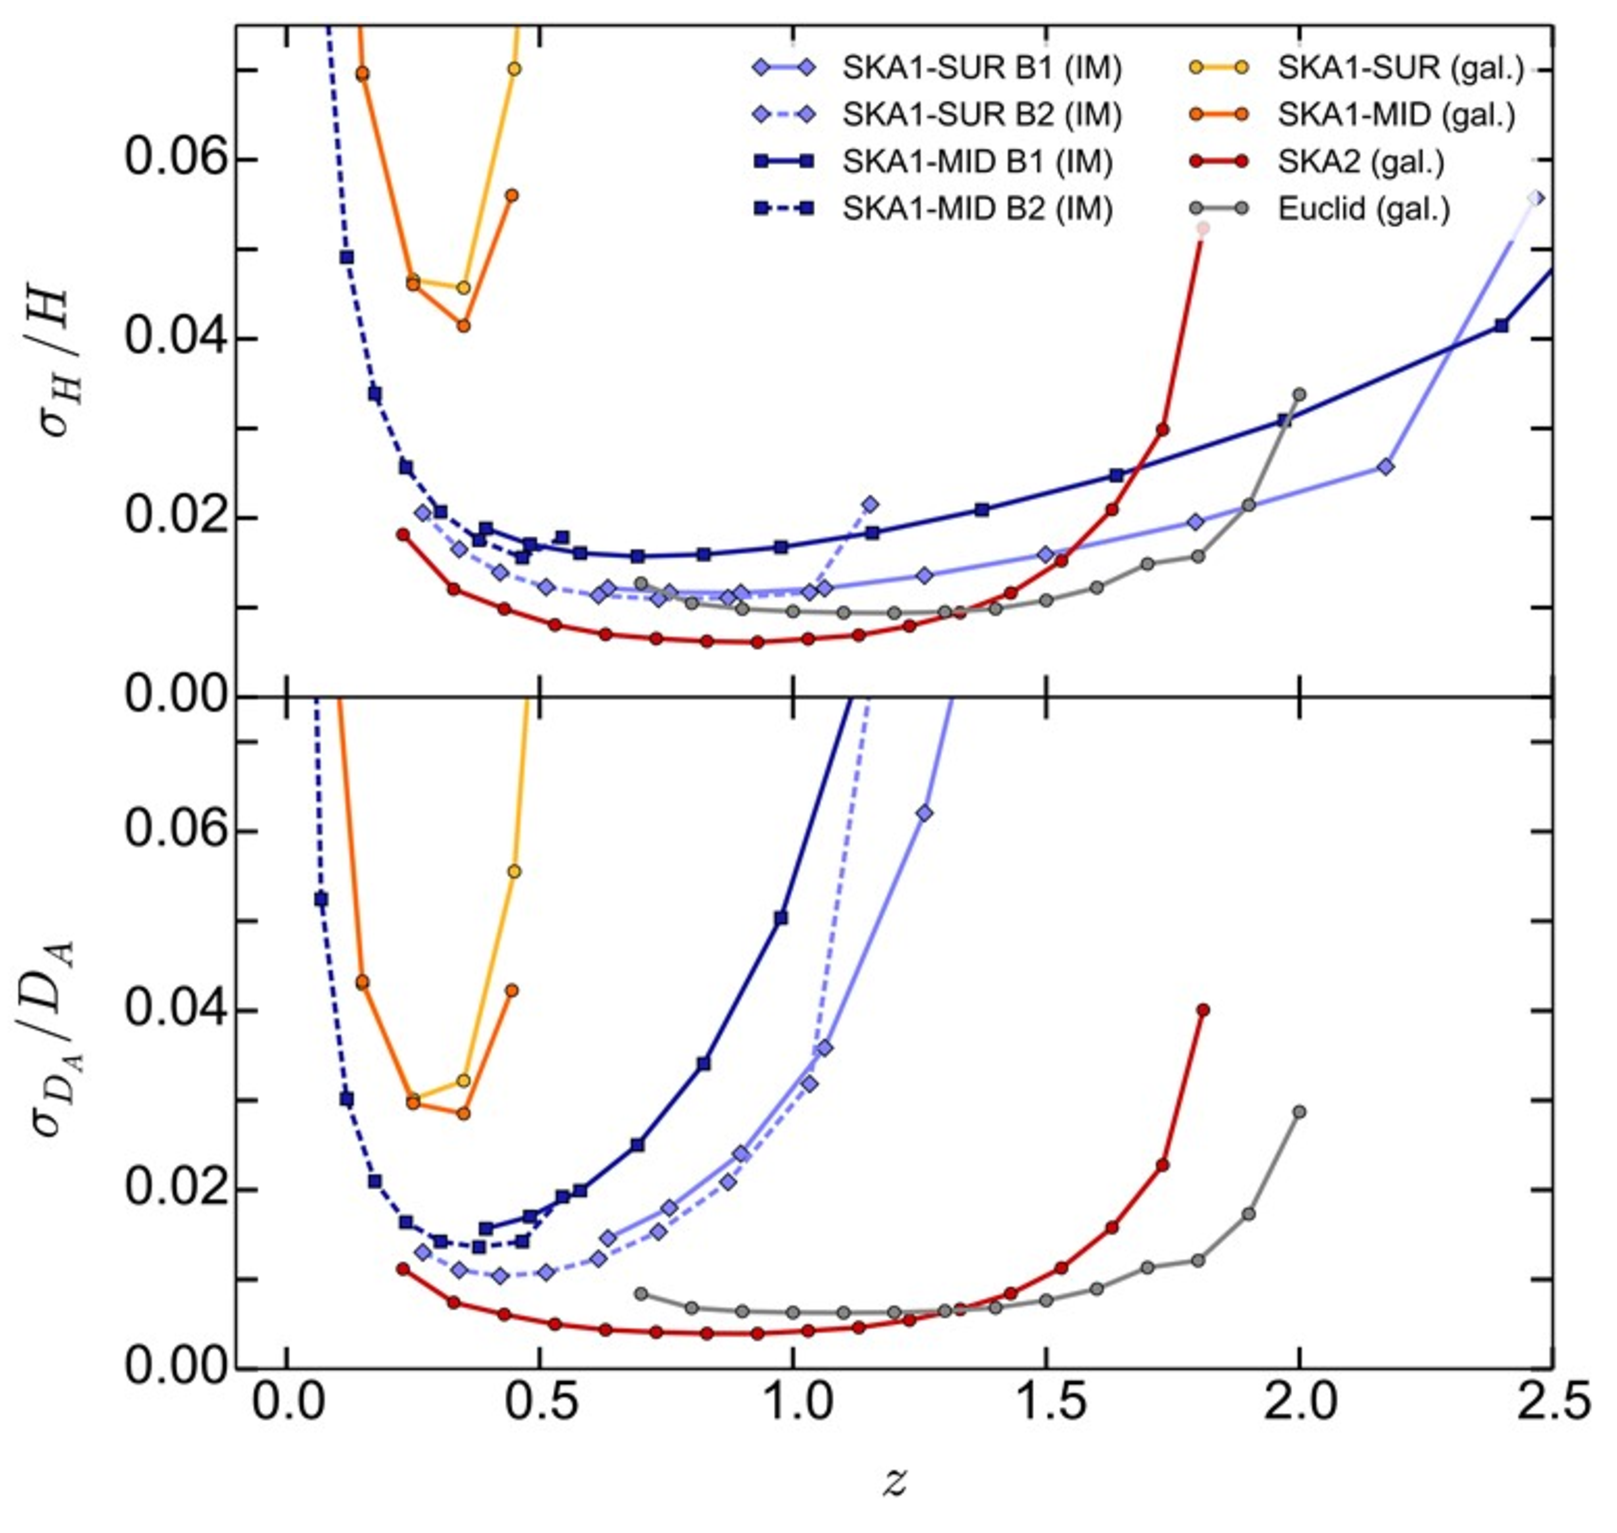
\includegraphics[width=1.0\linewidth]{cosmology/BAO_constraint.eps} 
%   \vspace{10pt}
 \end{center}
 \end{minipage}
 \begin{minipage}{0.52\hsize}
 \begin{center}
 \vspace{2.7cm}
   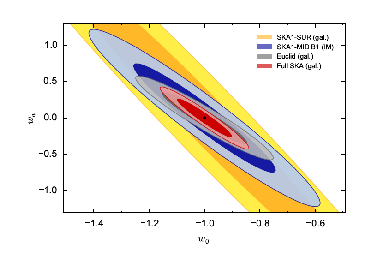
\includegraphics[width=1.0\linewidth]{cosmology/f2.eps} 
%  \vspace{-15pt}
 \end{center}
 \end{minipage}
  \caption{(左図)様々なBAO観測計画での$H$および$D_{\rm A}$の決定精度。 
(右図) 暗黒エネルギー状態方程式パラメータ$(w_0,w_a)$の決定精度。
比較のため、Euclidによる銀河サーベイ計画の感度もプロットしている。\citep{Bull:2015nra}
\label{fig:BAO fig}} 
\end{figure}
%%%%%%%%%%%%%%%%%%%%%%%%%%%%%%%%%%%%%%%%%%%%%%%%%%%%%%%%%%%%%%%%%%%%%%%%%%%%

BAOの振動スケールの測定は、主に銀河の赤方偏移探査から銀河のクラスタリング解析を行うことで行われる。\cite{2005ApJ...633..560E}によってSDSSのLRG(Luminous Red Galaxy)サンプルの二点相関関数の解析によって近傍の宇宙大規模構造において最初にBAOが検出された。実際に観測されるBAOスケールは天球面上の角度:
\begin{equation}
 d(z) = r_{\rm s}/D_{\rm V}(z),
\end{equation}
で与えられる。但し、$D_{\rm V}$は
\begin{equation}
 D_{\rm V}(z) = \left((1+z)^2D_{\rm A}^2(z)\frac{cz}{H(z)}\right)^{1/3}
\end{equation}
で与えられる。
ここで、$D_{\rm A}(z)\,, H(z)$はそれぞれ角径距離およびハッブル膨張率を表す。
これが観測されるBAOの振動スケールに一致するように宇宙論パラ
メータを決定するが、$D_{\rm V}(z)$だけを用いた宇宙論パラメータの推定には
パラメータ間の縮退が発生する。そこで、天球面方向と奥行方向のBAOの振動スケー
ルを別々に評価することで、それらの比である
\begin{equation}
 F(z) = (1+z)D_{\rm A}(z)H(z)/c
\end{equation}
を測定し、$D_{\rm V}(z)$と$F(z)$をあわせて宇宙論パラメータを推定すること
で上述の縮退を解くことができる。

BAOの振動スケールを様々な赤方偏移で測定することによって、より精密に宇宙論
パラメータを推定できる。中でもダークエネルギーのエネルギー密度とその状態
方程式パラメータ$w$の推定に利用される。現在の銀河の赤方偏移探査による
暗黒エネルギーの状態方程式パラメータの推定は、いわゆる宇宙定数と整合的
だが精度が良くない。状態方程式パラメータ(\eqref{eq:DE EOS def}, \eqref{eq:DE EOS}式)を
精密に測定することで、
暗黒エネルギーの正体の解明につながることが期待される。

\bigskip

図\ref{fig:BAO fig}左図はHI銀河赤方偏移サーベイ(gal)およびHI強度マッピングサーベイ(IM)を含む
様々なBAOの観測計画について達成可能な$H(z)$および$D_{\rm A}(z)$ の測定精度
を赤方偏移の関数として表したものである。Phase-1でのHI銀河赤方偏移サーベイでは
現在の可視光サーベイの推定精度と比較して同程度の推定精度であるのに対して、
強度マッピングサーベイでは観測するすべての赤方偏移においてHI銀河赤方偏移サーベイよりも
良い推定精度が期待される。また、Phase-2のSKAを用いたHI銀河赤方偏移サーベイではより広
い赤方偏移において1\%よりも良い推定精度で推定できると予想され、これは次世
代のEuclidなどのミッションと同程度の測定精度を達成できると期待さ
れる。これらのBAO観測計画による暗黒エネルギーの状態方程式パラメータの
推定精度が図\ref{fig:BAO fig}右図に示してある。

%%%%%%%%%%%%%%%%%%%%%%%%%%%%%%%%%%%%%%%%%%%%%%%%%%%%%%%%%%%%%%%%%%%%
\subsection{赤方偏移空間歪み}\label{cosmology.s2.ss2}
%%%%%%%%%%%%%%%%%%%%%%%%%%%%%%%%%%%%%%%%%%%%%%%%%%%%%%%%%%%%%%%%%%%%

遠方の天体までの距離は、その天体の宇宙膨張による後退速度に起因する赤方
偏移$z$と宇宙論パラメーターとに密接に関係している。その一方、その天体に
特有な特異運動(特異速度の動径成分)に起因する赤方偏移も存在する。この場
合、観測される赤方偏移の情報からだけでは本当の距離の見積もりを誤ること
になる。

この効果により、銀河の密度分布の相関を特徴付ける銀河の個数のパワースペ
クトル$P_{\rm g}^{\rm obs}(k,\mu,z)$は、真に正しい銀河のパワースペクト
ル$P_{\rm g}(k,z)$との間に、以下のようなズレが生じることが知
られている。
%%
\begin{eqnarray}
  \label{eq:Pobs}
  P_{\rm g}^{\rm obs}(k,\mu,z) = \left( 1 + \beta^2\mu^2\right) P_{\rm g}(k,z)
  \,,
\end{eqnarray}
%%
この式はカイザー公式と呼ばれ、線型近似の範囲内では妥当な近似式であ
ることが知られている。ここで、$\mu$は、着目している天体への視線方向と
波数ベクトル\mbox{\boldmath $k$}の間の方向余弦を表す。
ここで、その係数である赤方偏移空間変形パラメータ$\beta$は、後に説明する線型成長率指数$f$
および銀河密度と物質密度の間の違いを表すローカルな線型バイアスパラメータ$b$を
使って$\beta= f/b$と表される量である。
元来、真の銀河パワースペクトル$P_{\rm g}(k,z)$は、物質(ダークマタ—$+$バリオン)の
密度分布のパワースペクトル$P(k,z)$からズレていることが知られており、
先にも紹介したように、線型バイアスパラメター$b$を導入して、以下のように書き表される:
%%
\begin{eqnarray}
  \label{eq:biasedPgal}
  P_{\rm  g}(k,z)  = b^2(z) P(k,z),
\end{eqnarray}
%%
ここで、バイアスはスケールに依存しないと仮定している。
一方で、線型成長率指数$f(z)$は物質密度揺らぎの線形成長率$D(z)$を用いることで
以下のように定義される:
%%
\begin{eqnarray}
  \label{eq:growthrate}
  f(z) \equiv \frac{{\rm d} \ln D }{{\rm d} \ln a}
  \,,
\end{eqnarray}
%%
ここで$a(z)=1/(1+z)$はスケールファクターであり、$D(z)$は
今の場合次のようになる~\citep{Linder:2005in}:
%%
\begin{eqnarray}
  \label{eq:D-def}
  D(z) = a(z) \exp
    \left[
      \int_0^{a(z)}
      \left(
        \Bigl[\widetilde{\Omega}_{\rm m} (a')\Bigr]^\gamma - 1
      \right)
     \frac{d a'}{a'}
    \right]
   \,,
\end{eqnarray}
%%
但し、用いられた$ \widetilde{\Omega}_{\rm m}(a)$は、以下の定義である:
%%
\begin{eqnarray}
  \label{eq:OmegaEff}
  \widetilde{\Omega}_{\rm m}(a) = \frac{a^{-3}\Omega_{\rm m}}
{\sum_i\Omega_i 
\exp \left(
  3 \int_a^1 \left[
  w_i (a') + 1
              \right]
              \frac{d a'}{a'}
      \right)
   \,,
}
\end{eqnarray}
ここでの添字$i$は暗黒エネルギー、物質場、曲率、放射場を取り、
それぞれのエネルギー密度への寄与を表す。
このように定義した場合には、線型成長率指数$f$は
%%
\begin{eqnarray}
  \label{eq:fapprox}
  f(z) = \left[
        \widetilde{\Omega}_{\rm m}(z)
         \right]^{\gamma}
  \,,
\end{eqnarray}
のように表すことができる。
広く知られているように、一般相対論では$\gamma\simeq 0.55$である。
以下ではRSDの観測により、どのような宇宙論パラメータ
に対してどのような制限が得られるのかを簡単に紹介する。
 
\begin{description}
\item {\bf 暗黒エネルギーの状態方程式パラメータへの制限}

既に示したように、RSDを測定することで密度揺らぎの成長率$f$を観測から見積もることができる。
そのため、暗黒エネルギーと密接に関連していることからのその状態方程式パラメータ(\eqref{eq:DE EOS def}, \eqref{eq:DE EOS}式)の
推定に利用することができる。
将来のSKAによる観測により、この$2$つの
パラメータの精度よい情報が得られれば、宇宙定数とそれ以外の暗黒エネル
ギーのモデルを区別できることが期待されている。

\item {\bf 修正重力理論への制限}

\ref{cosmology.s1.ss1}節で述べてきたように、これまでに一般相対論を修正して、
暗黒エネルギーを説明しようとする試みが多数なされてきた。
%\eqref{eq:growthrate}式と
\eqref{eq:fapprox}式で導入された線型成長率指
数$f$の冪の$\gamma$は、修正重力理論に対して非常に鋭敏であることが知られている。
重力理論が一般相対性理論で記述される場合には$\gamma\approx 0.55$であるのに対し、
代表的な修正重力理論である$f(R)$重力理論では$\gamma\approx 0.40-0.43$、
DGPブレーンワールドモデルでは$\gamma\approx 0.68$程度の値をとることが示唆されてい
る~\citep{Linder:2005in}。この成長率指数を観測的に精度よく決める事により、修正
重力理論に対してする貴重な情報を得ることが出来る。
図~\ref{fig:RSD fig}左図はHI銀河赤方偏移サーベイ(gal)およびHI強度マッピングサーベイ(IM)による
RSD観測計画について、暗黒エネルギーの状態方程式パラメータ$w_0$と成長率指数$\gamma$の決定精度を
示したものである。図からわかるとおり、$\gamma$を制限することから
修正重力理論を区別するために十分な精度が期待できる。

%%%%%%%%%Figure%%%%%%%%%%%%%%%%%%%%%%%%%%%%%%%%%%%%%%%%%%%%%%%%%%%%%%%%%%%%%
\begin{figure}[t]
 \begin{minipage}{0.52\hsize}
 \begin{center}
%   \vspace{15pt}
   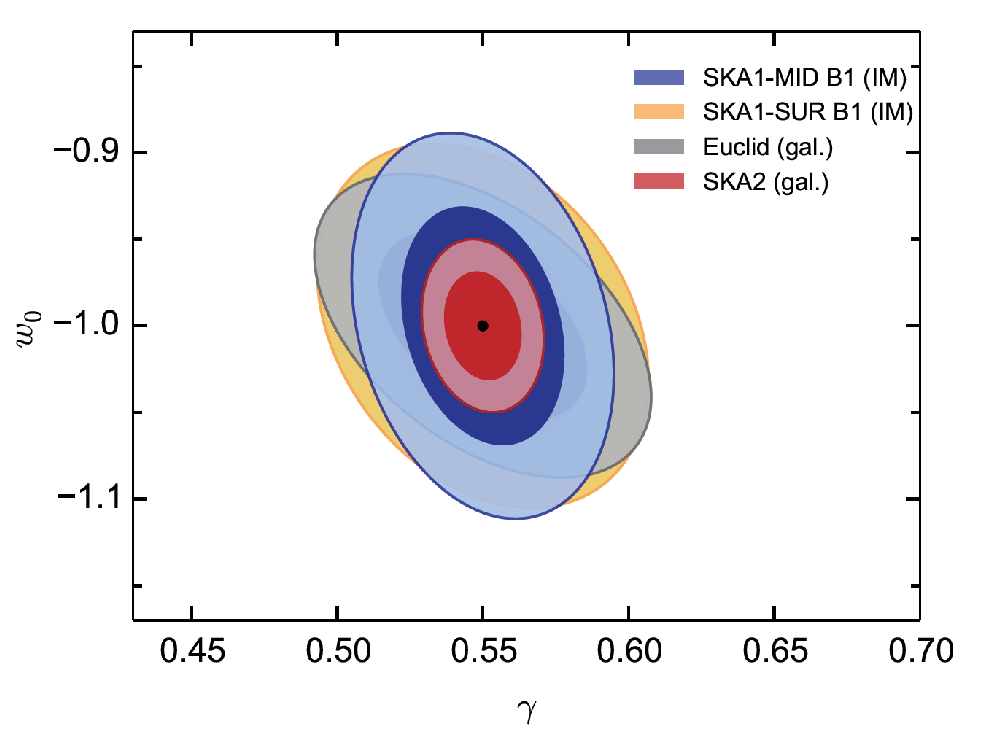
\includegraphics[width=1.0\linewidth]{cosmology/Fig3new.eps} 
%   \vspace{10pt}

 \end{center}
 \end{minipage}
 \begin{minipage}{0.52\hsize}
 \begin{center}
% \vspace{10pt}
   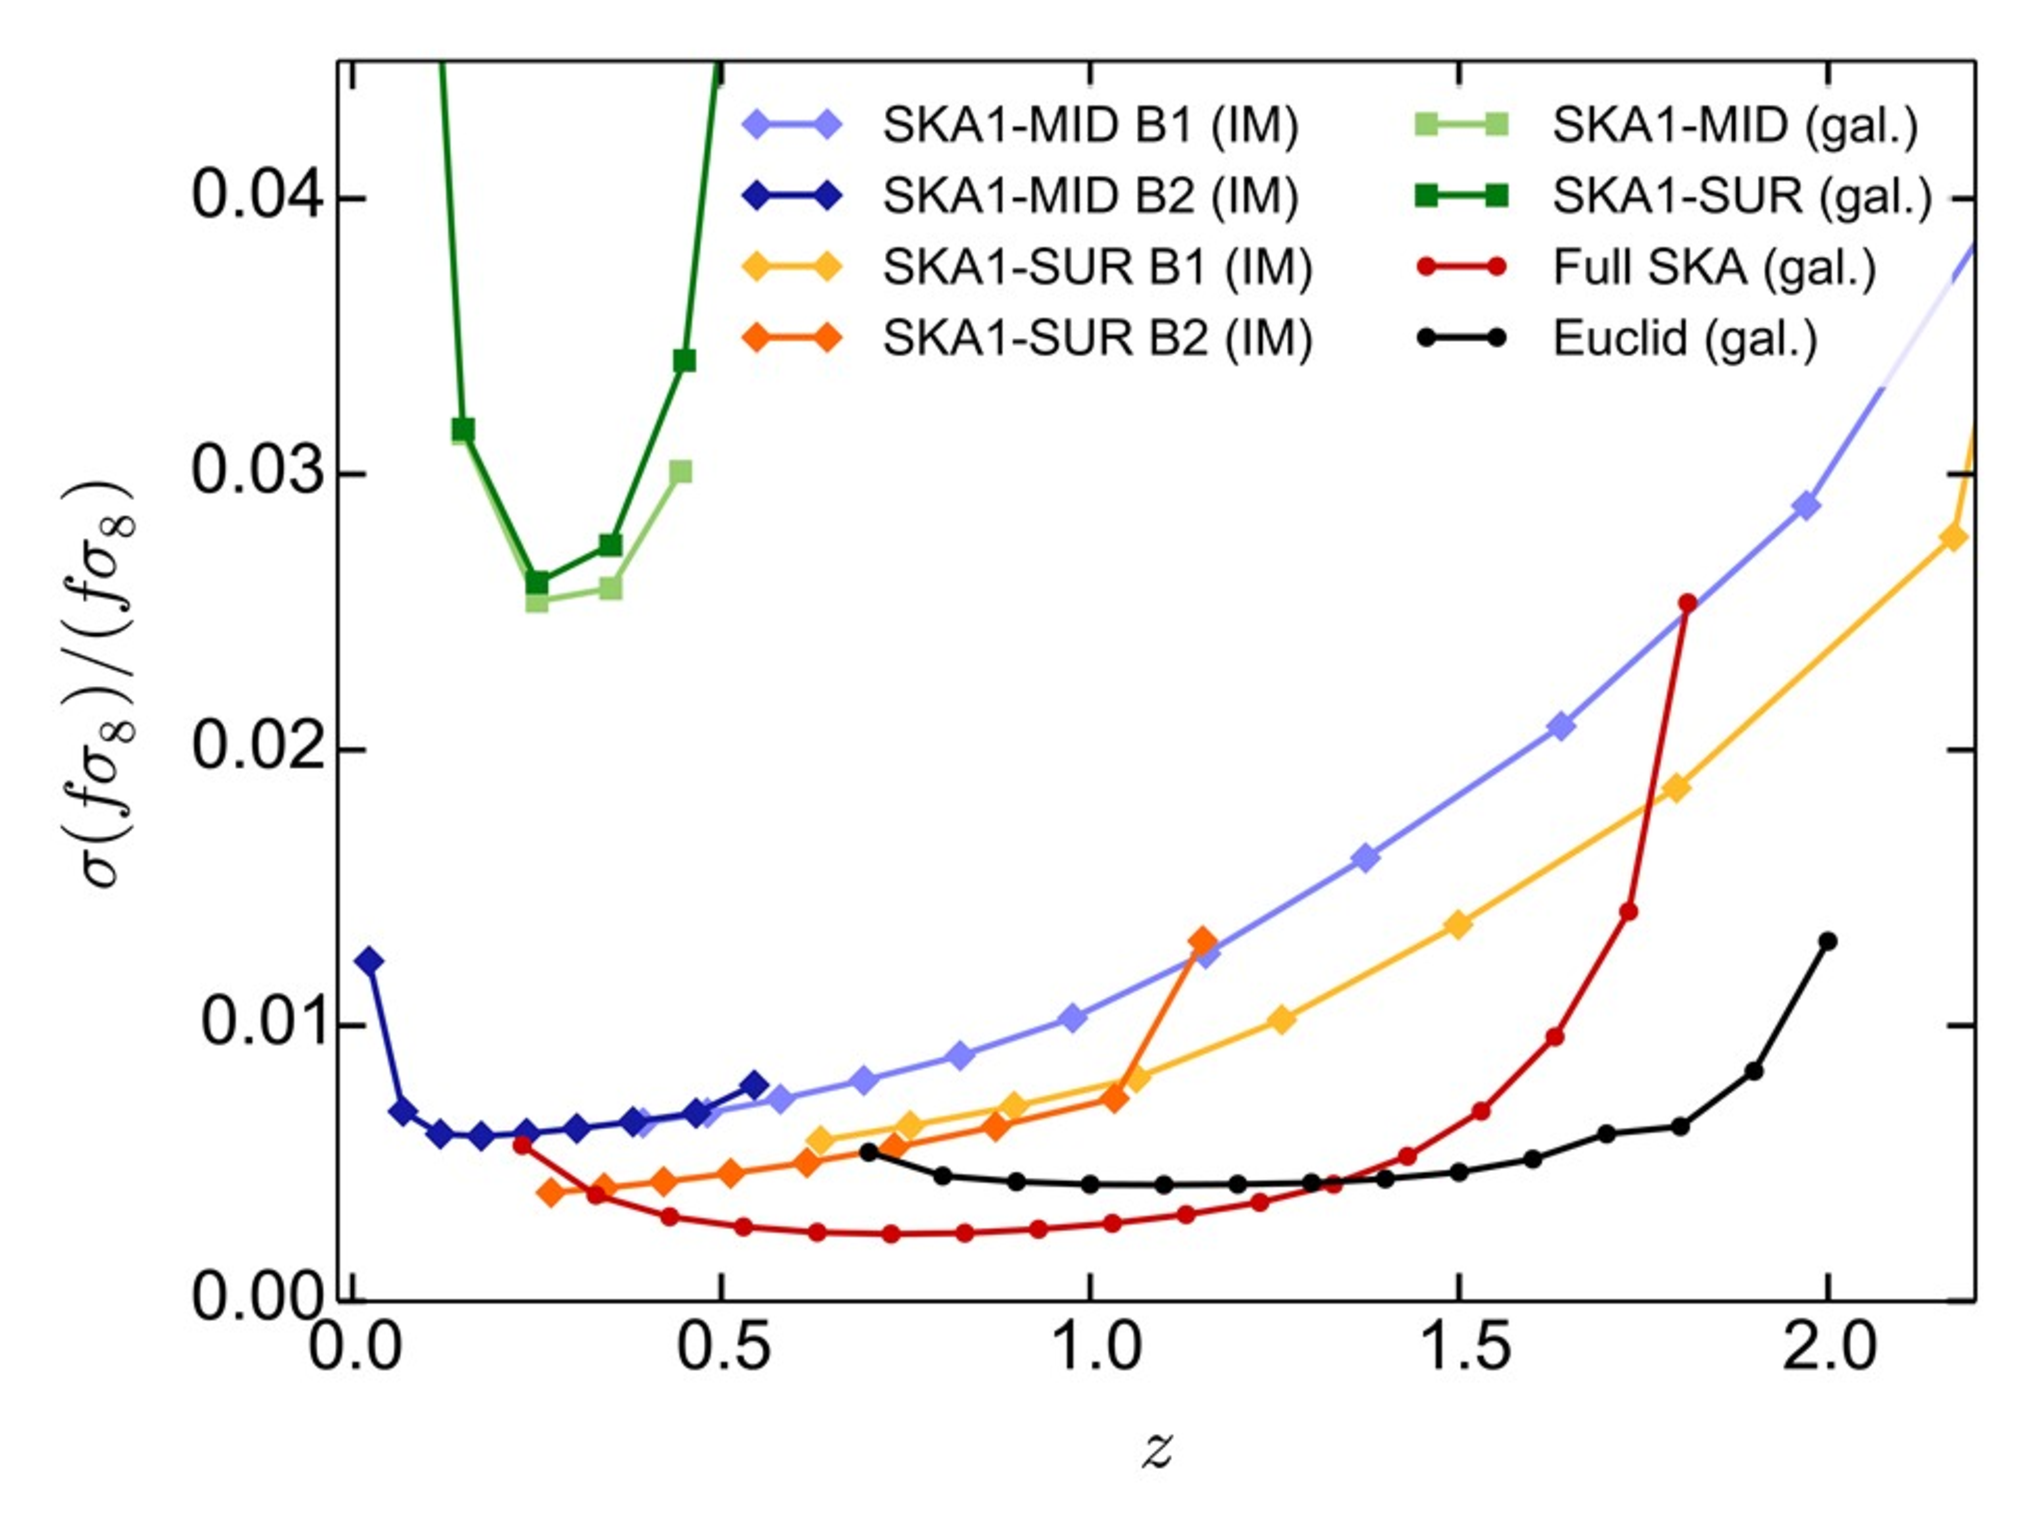
\includegraphics[width=1.0\linewidth]{cosmology/RSD_fs8.eps} 
%  \vspace{-15pt}
 \end{center}
 \end{minipage}
	\caption{(左図) 暗黒エネルギーの状態方程式パラメータ$w_0$および
	成長率指数$\gamma$の決定精度。
	(右図) $f\sigma_8$の決定精度。
	比較のため、Euclidによる銀河サーベイ計画の感度もプロットしている。\citep{Raccanelli:2015qqa}
	}
	\label{fig:RSD fig}
\end{figure}
%%%%%%%%%%%%%%%%%%%%%%%%%%%%%%%%%%%%%%%%%%%%%%%%%%%%%%%%%%%%%%%%%%%%%%%%%%%%

\eqref{eq:fapprox}式のように表せないような一般的な状況においては、質量揺らぎの分散の
平方根$\sigma_8$ (ここで$8$は半径$8h^{-1}$Mpcの球で平均した量であることを表す。)を用いて、
$f \sigma_8$および$b\sigma_8$の組み合わせについての制限を得る事により、
モデルを区別するという手法が取られる。
図~\ref{fig:RSD fig}右図に、赤方偏移$z$の関数として$f\sigma_8$の決定精度を示す。
\end{description}

%\bigskip

これまで示してきたように、RSDを観測することにより、宇宙論パラメーターを厳しく制限することができる。
特に、暗黒エネルギーのモデルパラメータへの制限はたいへん強力であり、暗黒エネルギーのモデルを
区別するために十分な感度を有している。
%ここでは、暗黒エネルギー密度が線型的に時間変化するモデルと、修正重力の単純なモデルについての解
%析結果を紹介してきた。
将来のSKAによるRSD観測により、暗黒エネルギーの正体が解明されることが期待される。


%%%%%%%%%%%%%%%%%%%%%%%%%%%%%%%%%%%%%%%%%%%%%%%%%%%%%%%%%%%%%%%%%%%%%%%%%%
\subsection{HI強度マッピング:前景放射}\label{cosmology.s2.ss3}
%%%%%%%%%%%%%%%%%%%%%%%%%%%%%%%%%%%%%%%%%%%%%%%%%%%%%%%%%%%%%%%%%%%%%%%%%%

既に述べたように、HI強度マッピングサーベイは個々の銀河を特定せず、
$1$つの大きなピクセルを用意し、そこに含まれる特定されない銀河群からの
中性水素$21$cm線を観測する。
これにより、大規模構造を$3$次元的に観測することが可能になる。
SKA-1 SURによる中性水素$21$cm観測により、$z<3$までの大規模構造を調べること
ができる。特に、宇宙論的な大規模構造の観測にはそれほどの分解能は不要であ
るので、視野の広い電波観測は都合がよい。また、$21$cm線には他の輝線と混同す
るおそれがない点も長所である。さらに干渉計による観測では、データを取得す
る際に周波数毎にビーム幅を合わせることが出来る点も、系統誤差を減らす点で
重要である。

ただし、これらは桁で大きい銀河系のシンクロトロン放射と自由-自由放射による前景放
射を除くことができればの話である。銀河系の放射は周波数方向になめらかであ
り、宇宙論的なシグナルは近似的には周波数毎に相関はないと期待されるので、
このことを用いて前景放射とシグナルを分離する手法が様々開発されている。
ここでは前景放射の差し引きの代表的な方法について紹介する~\citep{Wolz:2015sqa}。
これらの方法では、視線方向の長波長揺らぎ以外は統計誤差の範囲で再現でき
ることが分かっている。

\subsubsection{特異値分解法(SVD)}

この方法はGreen Bank Telescope (GBT)による観測で応用されている方法で、
主成分分析を経験的に発展させたものである\citep{2013MNRAS.434L..46S}。
観測機器による影響を減らすため、
データを二つのシーズンA,Bに分けて相互相関行列を考える。
これは時刻が違えばノイズ間の相関はないため、下に
述べる相互相関行列を元に前景成分を抽出する際にノイズの影響を減らすことができ
ると考えられているからである。相互相関行列は以下で与えられる。
\begin{equation}
 \bm{C}_{\rm AB} \equiv \left<
\vec{I}_{\rm A}(\theta)\left(\vec{I}_{\rm B}(\theta)\right)^{\rm T}
\right>
\end{equation}
ここで、$\vec{I}_{\rm A}(\theta)$はシーズンAでの$\theta$方向の電波強度を
あらわし、ベクトルの成分は各周波数での電波強度とする。括弧(
$\langle\cdots\rangle$ )で示した平均はピクセルでのサンプル平均とする。こ
の場合、$ \bm{C}_{\rm AB}$は実対称行列ではないので、対角化の代わりに特異
値分解$\bm{C}_{\rm AB} = \bm{U\Sigma V}^{\rm T}$を行い、$\vec{y}_{\rm
A}(\theta) = \bm{U}^{\rm T} \vec{I}_{\rm A}(\theta)$, $\vec{y}_{\rm
B}(\theta) = \bm{V}^{\rm T} \vec{I}_{\rm B}(\theta)$で定義すると、最大の
相互分散をもつ成分(これを前景放射とみなす)はシーズンAでは$y_{1}^{\rm
A}=\vec{u}_1^{\rm T} \vec{I}_{\rm A}$, シーズンBでは$y_{1}^{\rm
B}=\vec{v}_1^{\rm T} \vec{I}_{\rm B}$である。
また、これらの成分は無相関となる。今、21cmシグナルと前景放射は相関
がないと考えられていて、21cmシグナルに比べて前景放射の分散はずっと大きい
と思われているので、この成分を引くことで前景放射を除去できるというわけで
ある。
分散のもっとも大きい成分(p1
と する)は、例えばシーズンAでは$\vec{I}_{\rm p1}^{\rm A} = \vec{u}_1
\vec{u}_1^{\rm T} \vec{I}_{\rm A}$となるので、元のマップからこの成分を引
くことで前景放射の除去を行う。

\subsubsection{カルーネン$\cdot$レーベ分解}

この手法では具体的な前景放射モデルが必要である。CMBや大規模構造の研究で
使われてきており\citep{1995PhRvL..74.4369B,1996ApJ...465...34V}、最近
21cm線の研究に応用された\citep{2014ApJ...781...57S}。
相関行列がシグナル$\bm{S}$と前景放射$\bm{F}$の和で書けるとして、
$\bm{C}=\bm{S}+\bm{F} $とする。前景放射についてのみ白色化を行うと
\begin{equation}
\bm{F}^{-1/2} \bm{C} \bm{F}^{-1/2} = 
\bm{F}^{-1/2} \bm{S} \bm{F}^{-1/2} + \bm{I}
\end{equation}
を得る。この準白色化した相関行列を直交行列$\bm{O}$で対角化すると、
\begin{equation}
 \bm{F}^{-1/2} \bm{C} \bm{F}^{-1/2} = \bm{O}
(\bm{\Lambda}+\bm{I})\bm{O}^{\rm T}
\end{equation}
を得る。すなわち、直交行列の各列が$S/N$の大きい順に並んだ固有ベクトルと
なっている。この固有ベクトルを元にマップからシグナルの大きいものを抜き出せ
ばよいことになる。

\subsubsection{独立成分分析(FastICA)}

FastICAは観測されたmapを$\vec{I}(\theta)$、見積もりたいシグナルを
$\vec{s}(\theta)$としたときに、
\begin{equation}
 \vec{I} = \bm{A}\vec{s}
\end{equation}
というモデルを考え、$\bm{A}$と$\vec{s}$を同時に見積もる方法である。
そのために、各シグナル成分は独立であると仮定する。これは無相関より強い仮
定である。具体的には
\begin{equation}
 \vec{s} = \bm{W}\vec{I}
\end{equation}
という逆変換を考える際に、シグナルの各成分$s_i$の分布の非ガウス性が最大
になるように$\bm{W}$を構築すればよい。
CMBへの応用としては\cite{2002MNRAS.334...53M,2014ApJ...780...13I}、
21cm線観測への応用は\cite{2012MNRAS.423.2518C,2014MNRAS.441.3271W} がある。





%%%%%%%%%%%%%%%%%%%%%%%%%%%%%%%%%%%%%%%%%%%%%%%%%%%%%%%%%%%%%%%%%%%%%%%%%%
\subsection{HIトポロジー}\label{cosmology.s2.ss4}
%%%%%%%%%%%%%%%%%%%%%%%%%%%%%%%%%%%%%%%%%%%%%%%%%%%%%%%%%%%%%%%%%%%%%%%%%%

トポロジーは、宇宙の大規模構造を探り、
初期密度揺らぎの非ガウス性をテストするために当初導入された。
宇宙論パラメータの推定や銀河進化モデルへの制限などにも応用されている。
閾値を超える密度を持つ領域の幾何学は数学的には、ミンコフスキー汎関数を用いて
特徴付けられることが知られている~\citep{2008MNRAS.385.1613H}。
密度揺らぎ$\delta$およびその標準偏差$\sigma_0\equiv\langle\delta^2\rangle^{1/2}$を
用いることで、与えられた閾値$\nu =\delta /\sigma_0$を超えた等密度面の
ミンコフスキー汎関数は以下の$4$つ定義できる:
体積$V_0(\nu )$、表面積$V_1(\nu )$、平均密度$V_2(\nu )$、オイラー数$V_3(\nu)$である。
この中でも、オイラー数$V_3(\nu )$はジーナス(Genus)と呼ばれる量$G(\nu)$と
$V_3(\nu )=2-2G(\nu )$と関連している。
ジーナスは、考えている領域に存在する穴の数から孤立した領域の数を引いた量として定義される。
密度揺らぎが厳密にガウス分布に従う場合には、全てのミンコフスキー汎関数は
解析的に解かれており、
特に単位体積あたりのジーナス$G(\nu )$は次のように表す事が出来ることが知られている:
\begin{equation}
G(\nu)={\cal A}\left( 1-\nu^{2}\right) e^{-\nu^{2}/2},
\label{eq:genus}
\end{equation}
ここで、${\cal A}$は密度揺らぎ$\delta$のパワースペクトルを用いて得られる振幅である。
密度揺らぎのガウス分布からのどのようなズレも非ガウス性の証拠となりえるとともに、原始非ガウス性を
制限する手法となる。
原始非ガウス性はあらゆる高次モーメントによっても引き起こされることから、この研究は
これまでよく行われてきた$3$点相関関数つまりはバイスペクトルによる手法と相補的であると言える。
21cm線マップから得られるミンコフスキー汎関数は、低赤方偏移の大規模構造だけでなく、
高赤方偏移の再電離期における中性水素の分布の分布をも特徴付けることができる。
宇宙論の文脈の中で場の幾何学的性質を探るのが有効な手段となる分野は、以下の様なものが挙げられる。

\begin{description}
\item {\bf 原始非ガウス性 }

\ref{cosmology.s1.ss1}節で既に述べたように、原始非ガウス性は初期宇宙に対して深い理解を与えることができる。
初期密度揺らぎが\eqref{eq:fNL def}式で与えられる場合、
ジーナスは厳密なガウス分布の場合の\eqref{eq:genus}式からずれる。
ジーナスのガウス分布からのズレは、$2$次まで展開することで次のように得ることができる:
\begin{equation}
\Delta(\nu)\equiv \delta\left (\frac{G}{\cal A}\right) =-e^{-\nu^{2}/2}\biggl[\left( S_{\rm pri}^{(1)}-S_{\rm pri}^{(0)}\right) H_{3}(\nu )+\left( S_{\rm pri}^{(2)}-S_{\rm pri}^{(0)}\right) H_{1}(\nu ))\biggr]\sigma_{0},
\end{equation}
ここで、$H_n$はエルミート多項式であり、$S_{\rm pri}^{(a)}$は歪度パラメータと呼ばれる量である~\citep{2006ApJ...653...11H}。
$S^{(0)}_{\rm pri}$は揺らぎの歪度を表しているのに対し、$S^{(1)}_{\rm pri}$および$S^{(2)}_{\rm pri}$はその微分と関連する量であることから
\eqref{eq:fNL def}式に現れる非線形パラメータ$f_{\rm NL}$に依存している。
よって、これを測定することに事により、$f_{{\rm NL}}$への制限を得る事が出来る。
SKAでは$\sigma(f_{\rm NL})=20$程度の制限が予想される(図\ref{fig:fnl})。
原始非ガウス性が\eqref{eq:fNL def}式で書けない場合であってもジーナスに影響が及ぶことから
HIトポロジーは一般的な原始非ガウス性を制限しうる。

\item {\bf 暗黒エネルギーと修正重力理論 }

大規模構造のトポロジーは構造の成長と関係付けることができる。
実際、線形成長のみを考えるときには\eqref{eq:genus}式の${\cal A}$は保存し、
スムージングスケールを$R_{\cal G}$としたとき、
${\cal A}_{\rm Y}(z,R_{{\cal G},{\rm Y}})R_{\rm Y}^{3}={\cal A}_{\rm X}(R_{{\cal G},{\rm X}})R_{{\cal G},{\rm X}}^{3}$
なる関係が成り立つことが期待される~\citep{Park:2009ja}。
ここで、Xは真の宇宙論パラメータを表すのに対し、Yは採用した宇宙論パラメータを表し、一般に両者は異なっていてよい。
異なる宇宙論模型のスムージングスケール$R_{\cal G}$は、$(R_{{\cal G},{\rm X}}/R_{{\cal G},{\rm Y}})^{3}=(D_{\rm A}^{2}/H)_{\rm X}/(D_{\rm A}^{2}/H)_{\rm Y}$
を通じて結びつけられている。
%ここで、$D_{\rm A}$および$H$は角径距離およびハッブル膨張率を表す。
この効果を用いることで、大規模構造のトポロジーは標準ものさしとして用いる事ができ、暗黒エネルギーモデルへの制限を与える事が出来る。
また、修正重力理論を考える場合、揺らぎの成長率が一般相対論の場合と異なり、スケール依存性を持つことが知られている。
%その結果、ジーナスカーブに変更が加えられることになる。
暗黒エネルギーモデルへの制限と同様の理由で、修正重力理論のモデルへの制限も行う事が出来る。


\item {\bf 再電離 }

トポロジー解析は宇宙再電離の詳細な過程に対して直接的で鋭敏なプローブを与える。
トポロジーの定量的な観測量としてHIの密度等高線のジーナスを用いることで、
銀河間物質の再電離過程は次の4つのフェーズに分離することができる:
(i)再電離前、(ii)再電離開始後HII領域の重なり合いが始まる前、 (iii)重複期、 (iv)重複後、である。
(i)のフェーズでは、HIの分布は原始密度揺らぎを反映している。
そのため、ジーナスカーブはガウス分布と整合的であり、トポロジーはHI密度の
線形発展に対して変わらない。
(ii)は孤立したHIIバブルによるトポロジーによって特徴付けられる。
このフェーズの初期では、HIIバブルが徐々に増えて行くため、ジーナスカーブ
の振幅も徐々に増えて行く。
しかし、バブルの重なり合いが起きる(iii)ではジーナスカーブの振幅は徐々に減少していく。
(iv)では銀河間物質はほとんどイオン化しており、ジーナスカーブの成長は孤立した中性水素領域の数の
減少と整合的になる。
このように、ジーナスは中性水素領域のトポロジーの時間発展を追う事ができ、
さらに、再電離の異なる段階の赤方偏移を決定できるため、再電離シナリオの区別に
応用する事が出来ると考えられる~\citep{2014JKAS...47...49H}。
\end{description}


%%%%%%%%%%%%%%%%%%%%%%%%%%%%%%%%%%%%%%%%%%%%%%%%%%%%%%%%%%%%%%%%%%%%%%%%%%
\subsection{超地平線スケール宇宙論}\label{cosmology.s2.ss5}
%%%%%%%%%%%%%%%%%%%%%%%%%%%%%%%%%%%%%%%%%%%%%%%%%%%%%%%%%%%%%%%%%%%%%%%%%%

非常に大きなスケールに隠されている宇宙論的な情報は非常に重要になりえる。
大スケールでは構造の非線形発展を安全に無視することができるため、
揺らぎの発展は線形領域に留まっている。
また、物理過程はほとんど重力的な相互作用によって記述され、宇宙物理的な複雑な
プロセスを考慮に入れる必要がない。
そのような意味で、大スケールを観測することで非常にクリーンな探査が可能である。

大スケールは精密な理論予測が容易であるが、大スケールを観測することは非常に難しい。
大スケールに対応するような非常に小さなフーリエモードを探査するためには、
大角度を観測するだけでは不十分であることに注意する。
天球面上でどれだけ大スケールを観測しても、$3$次元の意味で観測しうるスケールは
視線方向成分で制限されてしまう。つまり、十分深いサーベイが必要がある。
二つ目の問題としては宇宙の単一性による有限サンプルから現れるノイズ:コズミックバリアンス(Cosmic Variance; CV)である。
どれだけ大きな体積を持ってきても観測体積内に含まれる天体が少数であれば、
その数で制限されてしまう。
SKAはこの状況を打破しうる観測であり、大スケールに関する研究を大いに推し進めることができる~\citep{Camera:2015yqa}。


%%%%%%%%%Figure%%%%%%%%%%%%%%%%%%%%%%%%%%%%%%%%%%%%%%%%%%%%%%%%%%%%%%%%%%%%%
\begin{figure}[t]
 \begin{minipage}{0.53\hsize}
 \begin{center}
%   \vspace{10pt}
   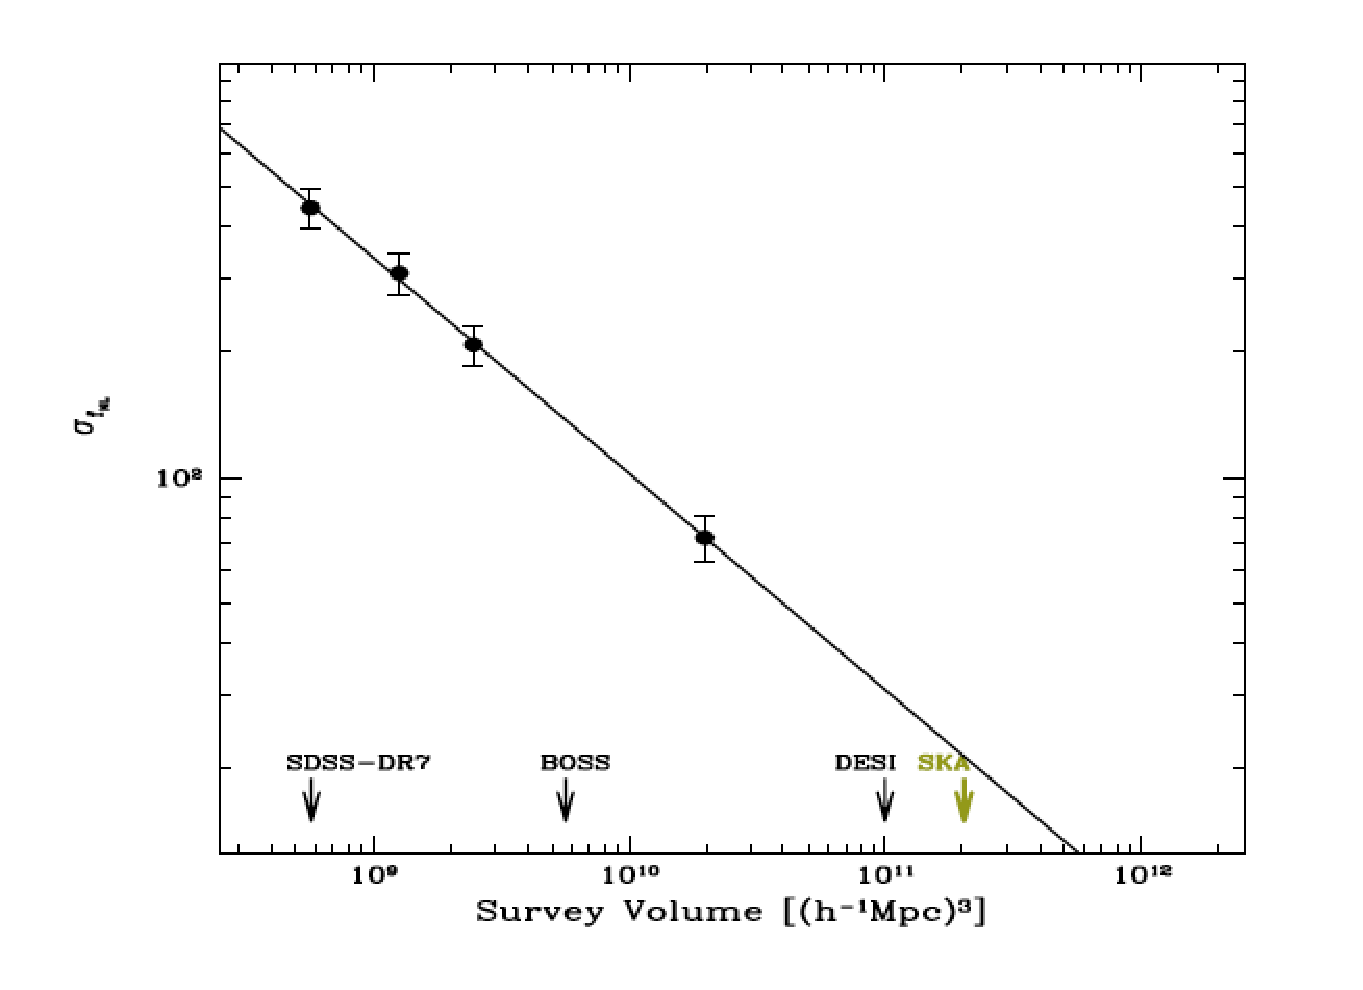
\includegraphics[width=1.0\linewidth]{cosmology/fnl.eps} 
%   \vspace{10pt}
   \caption{ジーナス統計を用いた$f_{\rm NL}$の決定精度。%SKAでは$2\times 10^{11}(h^{-1}{\rm Mpc})^{3}$のサーベイ体積を仮定。
}
\label{fig:fnl}
 \end{center}
 \end{minipage}
 \begin{minipage}{0.51\hsize}
 \begin{center}
   \vspace{5pt}
   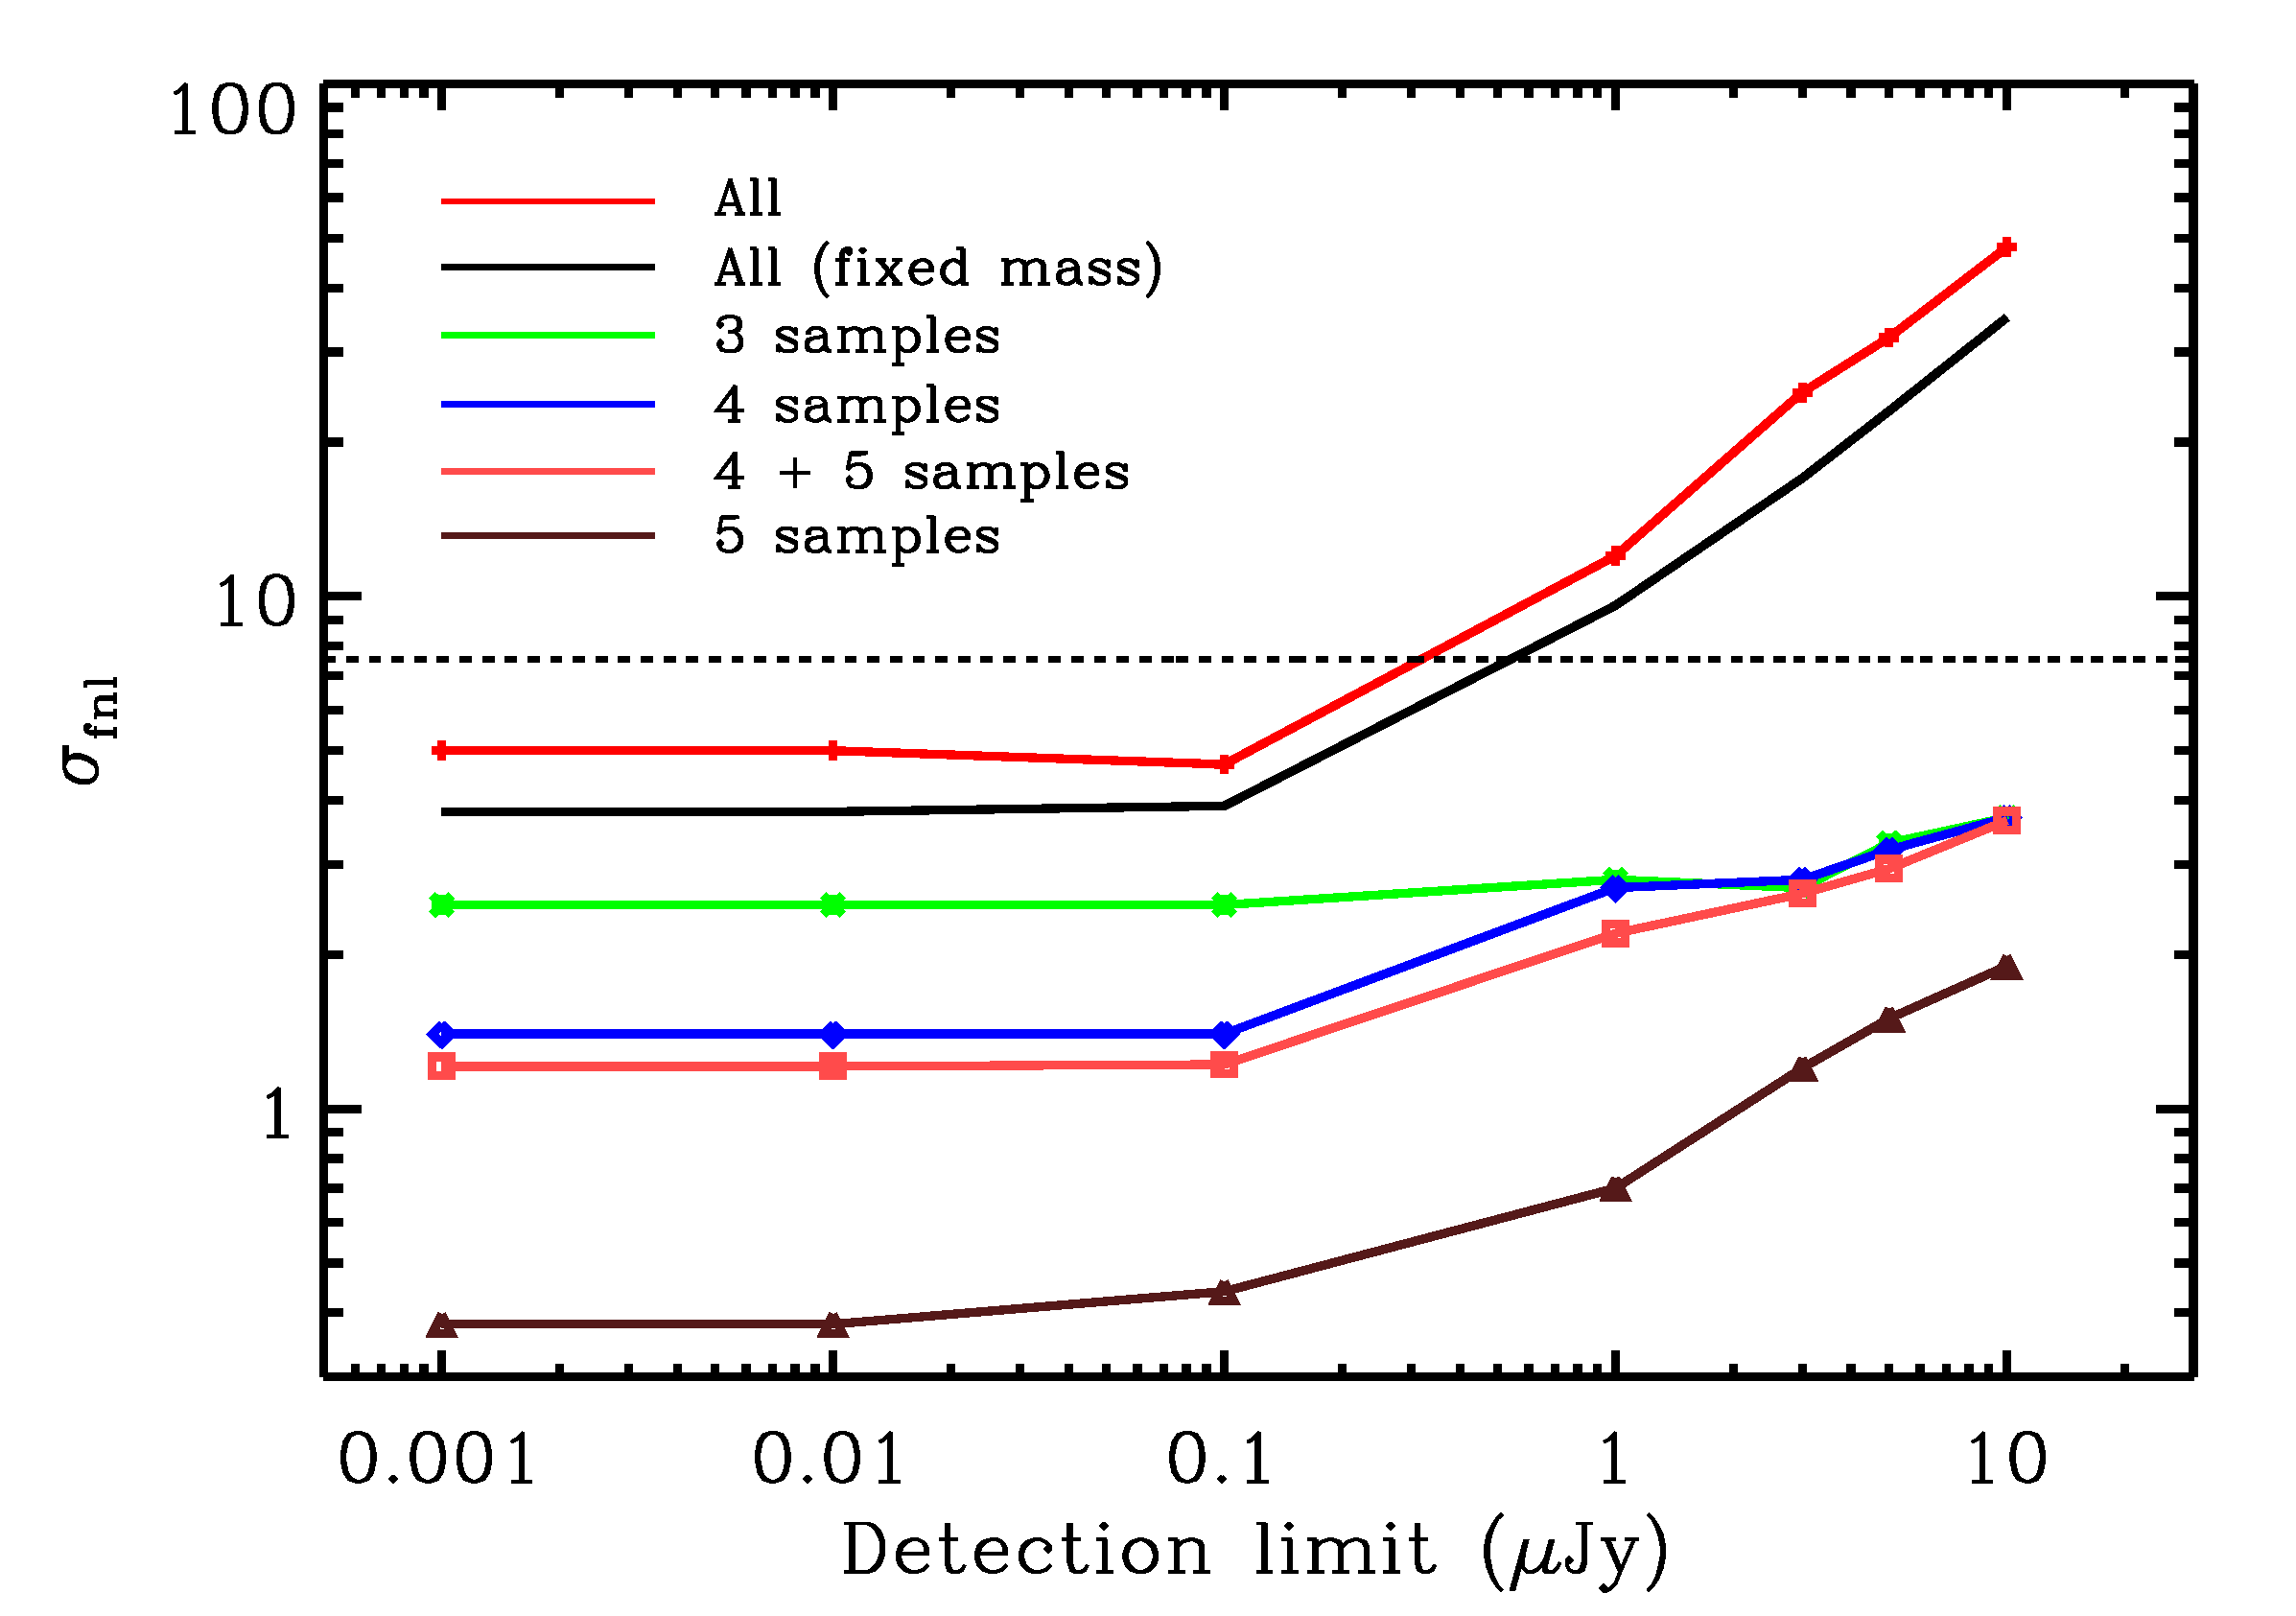
\includegraphics[width=1.0\linewidth]{cosmology/fig5.eps} 
%  \vspace{-15pt}
  \caption{マルチトレーサー法を用いた場合の$f_{\rm NL}$の決定精度~\citep{Ferramacho:2014pua}。
}
\label{fig:Ferramacho}
 \end{center}
 \end{minipage}
\end{figure}
%%%%%%%%%%%%%%%%%%%%%%%%%%%%%%%%%%%%%%%%%%%%%%%%%%%%%%%%%%%%%%%%%%%%%%%%%%%%


%%%%%%%%%%%%%%%%%%%%%%%%%%%%%%%%%%%%%%%%%%%%%%%%%%%%%%%%%%%%%%%%%%%%%%%%%
%=======================================================================%
\subsubsection{宇宙論的な大スケールを探査する重要性}
%=======================================================================%
%%%%%%%%%%%%%%%%%%%%%%%%%%%%%%%%%%%%%%%%%%%%%%%%%%%%%%%%%%%%%%%%%%%%%%%%%

%これまでにない規模の大体積を探査することにより、
%「インフレーションを起こしたメカニズムは何か?」
%「大スケールにおいて一般相対論は実現しているのか?」
%というような宇宙論における基礎的な疑問に答えていくことができる。
%
\ref{cosmology.s1.ss1}節で述べたように、原始非ガウス性はインフレーション模型を決定付けるために有用である。
現在最も厳しい原始非ガウス性の制限はPlanck衛星によるものであるが、将来のCMB観測を用いたとしても
Planck衛星の結果以上に改善することは難しい。
原始非ガウス性を制限する新しいフロンティアは物質分布の大体積のサーベイである。
%
同様に、宇宙論的スケールにおける一般相対論のテストも大規模構造の観測によって行うことができる。
加えて、より大スケールを観測し、統計を稼ぐことにより、暗黒エネルギーや修正重力理論の
厳しい制限を与えることができる。
以下、SKAサーベイで期待される成果についてより具体的に述べる。

\begin{description}
\item {\bf 一般相対論効果 }

一般相対論的効果は、過去の光円錐上において数密度や輝度温度揺らぎを観測する際に現れる。
これまでの解析では、ニュートン近似への標準的な補正として赤方偏移歪みと重力レンズによる増幅効果
のみを部分的に取り入れてきた。
しかし、これらの効果は十分小スケールでのみ重要になってくる。
将来の広範かつ深いサーベイにおいては、宇宙物理学的な複雑なプロセスは無視できても
全ての一般相対論的補正を含むような精緻な模型を用いることが
重要になる~\citep{Yoo:2010ni,Bonvin:2011bg,Challinor:2011bk,Bruni:2011ta}。
%その特徴の一つとして、一般相対論効果を含む2点相関関数をルジャンドル陪関数で展開したときには、
%標準的な解析ではゼロであったパリティ奇のモードが寄与することが指摘されている。

\item {\bf 原始非ガウス性 }

大スケールを探査することで宇宙原始揺らぎの重要な情報を得ることができる。
これまで原始揺らぎの非ガウス性を探る最もよいプローブはCMB温度揺らぎのバイスペクトルであった。
しかし、原始非ガウス性は、背後にある物質分布のバイアスに対してスケールおよび赤方偏移依存性を付与する
ことが明らかとなった\citep{Dalal:2007cu,Matarrese:2008nc,Schmidt:2010gw,Desjacques:2008vf}。
原始非ガウス性がないときの大スケールのバイアスを$b$と書いたとき、
\eqref{eq:fNL def}式で与えられる原始非ガウス性による補正項は次のように書ける:
\begin{align}
	\Delta b(z,k)=3[b(z)-1]\frac{\Omega_{\rm m}H_0^2\delta_c}{k^2T(k)D(z)}f_{\rm NL}
	\,.\label{eq:scale dependent bias}
\end{align}
ここで、$\delta_c$は崩壊時の物質揺らぎの臨界値、$T(k)$は遷移関数、$D(z)$は密度揺らぎの線形発展因子である。
原始非ガウス性の効果により、パワースペクトルは大スケールで$k^{-2}$として振舞う。
これは一般相対論的効果が効くスケールと一致しており、原始非ガウス性の精密な予言のために一般相対論的効果を
適切に取り入れることが必要である。


\item {\bf 修正重力理論 }

一般相対論は実験室や太陽系スケールでは精緻にテストされてきたが、宇宙論スケールではいまだ弱い制限しかない。
暗黒エネルギーの文脈において大スケールにおける一般相対論のテストは非常に注目されている。
\ref{cosmology.s1.ss1}節で述べたように、暗黒エネルギーの代替要素としての修正重力理論はこれまで非常に多く提案されて
おり、これらの多くは暗黒エネルギーの状態方程式(\eqref{eq:DE EOS def}式)を変更することから、
これを精密に探査することで模型を区別することができると期待されている。
修正重力理論の暗黒エネルギー以外の典型的な予言としては揺らぎの発展史への修正が挙げられる。
その中でも揺らぎの成長率は最も揺らぎの発展史に鋭敏であり、HI銀河赤方偏移サーベイや
HI強度マッピングサーベイによりRSD (\ref{cosmology.s2.ss2}節)を用いることで測定することができると期待されている。

\end{description}


%%%%%%%%%%%%%%%%%%%%%%%%%%%%%%%%%%%%%%%%%%%%%%%%%%%%%%%%%%%%%%%%%%%%%%%%%
%=======================================================================%
\subsubsection{宇宙論的な大スケールの観測手法}
%=======================================================================%
%%%%%%%%%%%%%%%%%%%%%%%%%%%%%%%%%%%%%%%%%%%%%%%%%%%%%%%%%%%%%%%%%%%%%%%%%

%%%%%%%%%%%%%%%%%%%%%%%%%%%%%%%%%%%%%%%%%%%%%%%%%%%%%%%%%%%%%%%%%%%%%%%%%
%=======================================================================%
\paragraph{再イオン化期後の強度マッピング}
%=======================================================================%
%%%%%%%%%%%%%%%%%%%%%%%%%%%%%%%%%%%%%%%%%%%%%%%%%%%%%%%%%%%%%%%%%%%%%%%%%

$21$cmパワースペクトルをモデル化する際、物質場とHIパワースペクトルの間の関係を決める
バイアス関数の定量化は難しい。
バイアスを理解するために、大規模構造の流体計算や$N$体計算の結果から擬似HIパワースペクトル
を抜き出す様々な手法が開発されている。
その中で、$k\lesssim 1\,h{\rm Mpc}^{-1}$のスケールではバイアスは定数に漸近
することが示されている~\citep{Villaescusa-Navarro:2014cma}。
バイアスの完全な特徴を掴むまでには至っていないが、十分大スケールでHIバイアスを定数だと
仮定することで、修正重力理論や原始非ガウス性の研究に応用することができる。

\begin{description}
\item {\bf スケールに依存するバイアスによる原始非ガウス性の探査 }

HIバイアスを通じて、原始非ガウス性を制限することができる~\citep{Camera:2013kpa}。
再イオン化後では、ほとんどの中性水素は銀河内にしか存在しないと考えられることから、
中性水素のパワースペクトルは銀河に付随する暗黒物質ハロー分布にバイアスされていると考えられる。
実際、視線方向の散乱および自己吸収を無視した場合、HI線放射はハローの微分数密度と関連付けることができ、
これによりバイアスを推定することができる。
SKA1-MIDを用いた場合の原始非ガウス性の決定精度は
$\sigma (f_{\rm NL})\sim 2$となる。
SKA2では$\sigma (f_{\rm NL})\lesssim 1$を達成できる。

\item {\bf バイスペクトルによる原始非ガウス性の探査 }
銀河に比べ、HIの物質分布へのバイアスは相対的に小さい。
そのため、線形バイアスおよび非線形バイアスの寄与を加えた樹形バイスペクトル
をHIのバイスペクトルとしてモデル化することができる。
高赤方偏移において原始密度揺らぎの寄与はより重要になる。
SKA 1-MIDでは$\sigma (f_{\rm NL})=45.7$であり、
SKA2においては$\sigma (f_{\rm NL})=6.6$まで改善する。
\end{description}


%%%%%%%%%%%%%%%%%%%%%%%%%%%%%%%%%%%%%%%%%%%%%%%%%%%%%%%%%%%%%%%%%%%%%%%%%
%=======================================================================%
\paragraph{再イオン化期における強度マッピング}
%=======================================================================%
%%%%%%%%%%%%%%%%%%%%%%%%%%%%%%%%%%%%%%%%%%%%%%%%%%%%%%%%%%%%%%%%%%%%%%%%%

原始非ガウス性は初期星形成銀河ハローのクラスター化にも影響を及ぼす。
再イオン化時に星形成銀河ハローは銀河間物質中にイオン化されたパッチの
ネットワークを形成することから、イオン化水素の分布には原始非ガウス性の
痕跡が残っていると期待される。
ここで、イオン化密度バイアスは再イオン化模型から導くことができる。
SKA1-LOWでは、この手法による原始非ガウス性への制限は$\sigma (f_{\rm NL})=7.4$となる。
full SKAを用いることができるならば制限は$\sigma (f_{\rm NL})=4.7$まで改善することができる~\citep{Mao:2013yaa}。


%%%%%%%%%%%%%%%%%%%%%%%%%%%%%%%%%%%%%%%%%%%%%%%%%%%%%%%%%%%%%%%%%%%%%%%%%
%=======================================================================%
\paragraph{マルチトレーサー法}
%=======================================================================%
%%%%%%%%%%%%%%%%%%%%%%%%%%%%%%%%%%%%%%%%%%%%%%%%%%%%%%%%%%%%%%%%%%%%%%%%%

大スケールでの統計解析はスケールに依存するバイアスを通じて非ガウス性を探査することに対して非常に有利だが、精度は本質的にCVによって制限される。\cite{Seljak:2008xr}によって異なるバイアスを持つ2つ以上の観測量を用いることでCVをうまく回避する方法が提案されている。これをマルチトレーサー法と呼ぶ。
この方法の基本的なアイデアとしては、少なくとも2つの異なるバイアスを持つ観測量を用意することでバイアスの比の決定精度についてはショットノイズだけによって決まるようにできることにある。\cite{Ferramacho:2014pua}においてこれをSKAの連続波サーベイに適用している。SKA1においてマルチトレーサー法を用いないと$\sigma (f_{\rm NL})=32$であるのに対し、用いることで
$\sigma (f_{\rm NL})\sim 2.9$まで改善する。
SKA2においては$\sigma (f_{\rm NL})\sim 0.7$にまで到達することができると期待されている。
図\ref{fig:Ferramacho}にフラックスカットの関数として$f_{\rm NL}$の決定精度を図示する。

\bigskip

ここまで示したように、SKAによって可能になる大スケールの観測によって、
「インフレーションを起こしたメカニズムは何か」、「大スケールにおいて一般相対論は実現しているか」
というような宇宙論における基礎的な疑問に答えることができるようになる。
特に、これまで最も厳しい制限を与えてきたCMBによる制限を凌ぐ制限を与えることが可能になる。
SKAが与えうる制限はEuclid衛星に代表される他波長の観測計画(\ref{cosmology.s1.ss2}節)と競合しているが、
これらのノイズの統計的性質はそれぞれに異なっていることから、それぞれの制限は相補的である。



%%%%%%%%%%%%%%%%%%%%%%%%%%%%%%%%%%%%%%%%%%%%%%%%%%%%%%%%%%%%%%%%%%%%%%%%%%
\subsection{弱重力レンズ}\label{cosmology.s2.ss6}
%%%%%%%%%%%%%%%%%%%%%%%%%%%%%%%%%%%%%%%%%%%%%%%%%%%%%%%%%%%%%%%%%%%%%%%%%%

%%%%%%%intro%%%%%%%%%%%%%%%%%%%%%%%%%%%%%%%%%%%%%%%%%%%%%%%%%%%%%%%%%%%%%%%%
SKAでは銀河探査を利用した弱重力レンズ探査に加え、
中性水素ガス21cm線の強度分布の観測を利用した手法も考えられており、
特に後者は銀河探査よりも大きな赤方偏移の時代の観測に利用できると期待されている。
本節では,これらSKAを利用した弱重力レンズ探査について以下で解説を行っていく。

%%%%%%%%%%%%%%%%%%%%%%%%%%%%%%%%%%%%%%%%%%%%%%%%%%%%%%%%%%%%%%%%%%%%%%%%%%%%
\subsubsection{銀河の弱重力レンズ効果の測定}
%
銀河に対する弱重力レンズ効果は、観測された銀河の形が歪む効果として観測される。
現在この銀河探査による弱重力レンズ効果の観測は、可視光による観測が先行しており、
CFHTLenS surveyなどで実際にその効果が精度良く観測されている~\citep{Heymans:2013fya}。
%
しかしSKAの様な電波領域における高視野,高解像度の観測が実現すれば、
従来可視光の領域であった弱重力レンズ探査を
電波観測によって行うことができるようになると期待されており、
現在その観測における問題点や解析手法に対する研究が精力的に行われている~\citep{Brown:2015vqa,Patel:2015cra}。

弱重力レンズ効果の観測においては、銀河の形状を解析する必要なら観測機器の角分解能に依存する。
SKAは他波長、特に光赤外観測計画(\ref{cosmology.s1.ss2}節)に比べ、角分解能は若干見劣りする。
しかし、SKAはほぼ全体にわたる広い立体角($\sim 3\pi$ steradian)を観測するとともに、
$z\gtrsim 2$のような大きな赤方偏移を持つ銀河を観測しうることから、他波長の観測と
競合するほどの性能を持つ。
%
例えば図\ref{fig:WL_fig1}の左図は、
SKAによって連続波を用いて銀河探査を行った場合に期待される弱重力レンズ効果によって生じる歪みの効果
(歪み場相関関数のパワースペクトル)とその測定エラーである。
光赤外による銀河探査計画であるEuclidと比較して、より大きな赤方偏移の銀河を多数観測することが
可能であり、その結果SKAを利用することで非常に精度よく歪み場の観測が可能であることがわかる。
%
また図\ref{fig:WL_fig1}の右図は
SKA2の弱重力レンズ効果の観測を行った場合に期待される、
物質(暗黒物質とバリオン)の密度パラメータ$\Omega_{\rm m}$、
及び質量揺らぎの分散の平方根$\sigma_{8}$に対する制限の図である。
%
特に質量揺らぎの分散$\sigma_{8}$は、密度揺らぎの成長を通して
暗黒エネルギーの性質に依存するため、
$\sigma_{8}$の精密な測定は正体不明の暗黒エネルギーの性質を調べる上で
きわめて重要であると言える。
%
%なおこの
解析結果によれば、SKA1-earlyでさえ、
現在の可視光による弱重力レンズ効果の観測と比較して
数倍程度強い制限を与えることができると期待できる。
またSKA1は光赤外将来計画DESと並び、
さらにSKA2のおいてはEuclidと比肩するほどの
観測性能を持つ。
SKAによる弱重力レンズ効果の観測が非常に強力であることが分かる。


%%%%%%%%%Figure%%%%%%%%%%%%%%%%%%%%%%%%%%%%%%%%%%%%%%%%%%%%%%%%%%%%%%%%%%%%%
\begin{figure}[t]
 \begin{minipage}{0.53\hsize}
 \begin{center}
   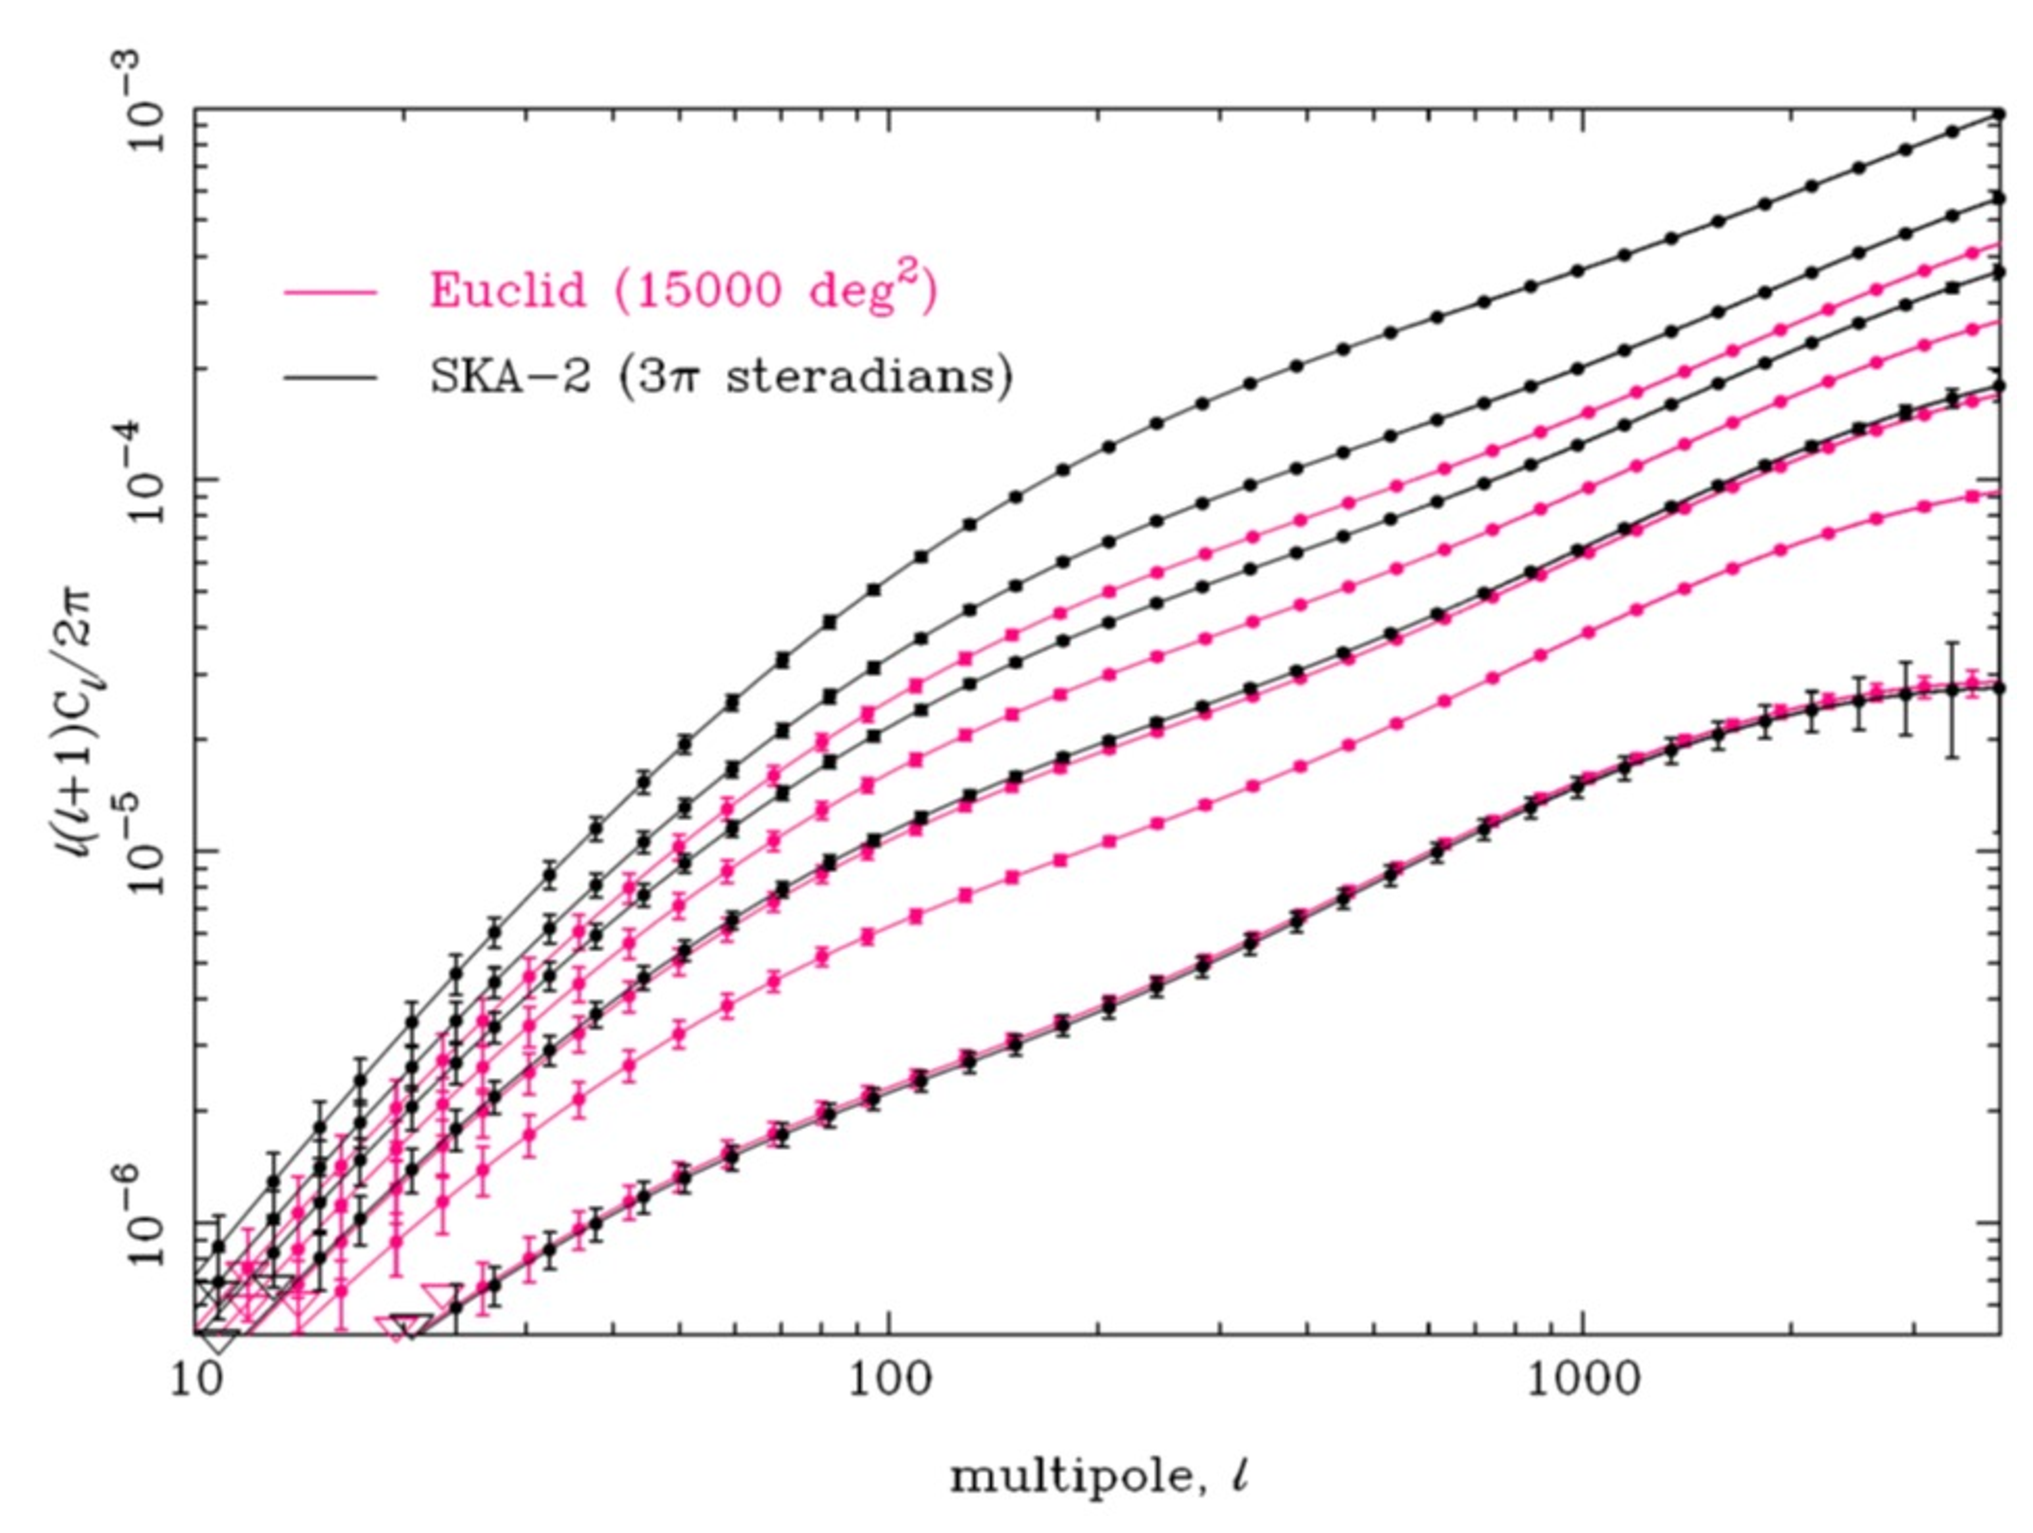
\includegraphics[width=1.0\linewidth]{cosmology/WL_power.eps} 
 \end{center}
 \end{minipage}
 \begin{minipage}{0.51\hsize}
 \begin{center}
   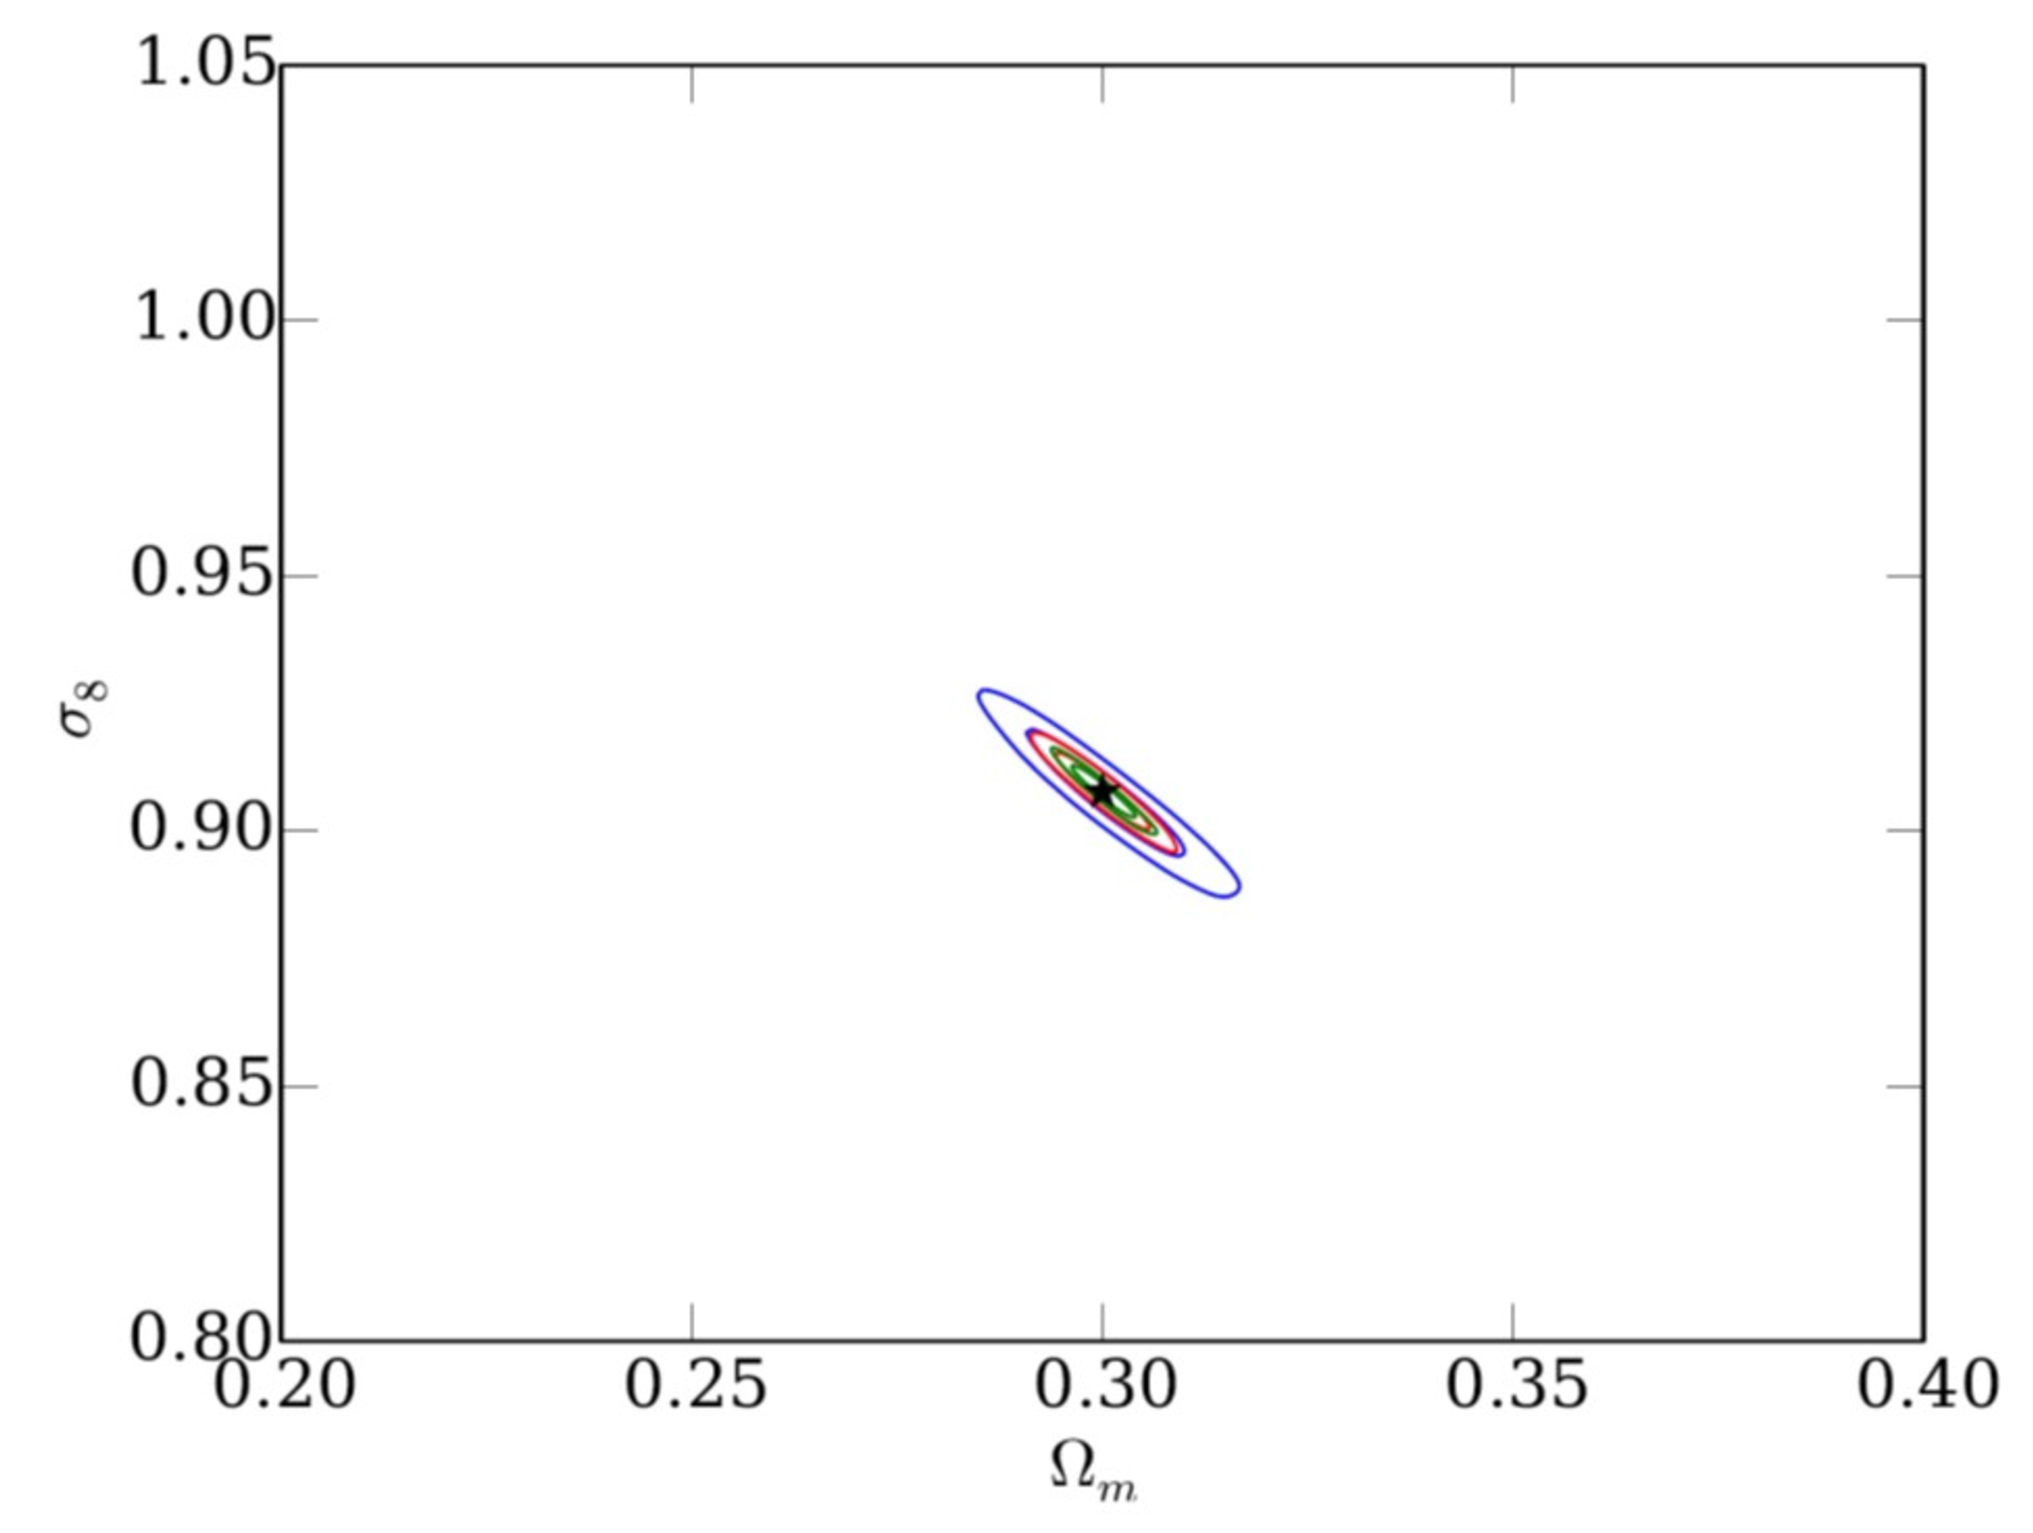
\includegraphics[width=1.0\linewidth]{cosmology/WL_constraint.eps} 
 \end{center}
 \end{minipage}
\caption{(左図) SKA2で期待される歪み場のパワースペクトルとその観測エラー
(各線は異なる赤方偏移におけるパワースペクトルであり、それぞれの実験に対し
赤方偏移ビンを$5$つに区切り、各赤方偏移ビンの幅は観測される銀河数が
同数になるように取られている。)。
比較のため、Euclidによる歪み場のパワースペクトルを赤線で示す。
(右図) SKA2の弱重力レンズ効果の観測を行った場合に期待される
$\Omega_{\rm m}$と$\sigma_{8}$の決定精度。
なお円の色の違いは観測する立体角の違いを表し、
それぞれ青線:$1000~{\rm deg}^2$、赤線:$5000~{\rm deg}^2$、緑線:$3\pi~{\rm steradian}$
の場合の制限である\citep{Brown:2015vqa}\label{fig:WL_fig1}。}
\end{figure}
%%%%%%%%%%%%%%%%%%%%%%%%%%%%%%%%%%%%%%%%%%%%%%%%%%%%%%%%%%%%%%%%%%%%%%%%%%%%
%%%%%%%%%Figure%%%%%%%%%%%%%%%%%%%%%%%%%%%%%%%%%%%%%%%%%%%%%%%%%%%%%%%%%%%%%
\begin{figure}[t]
 \begin{center}
%   \vspace{15pt}
   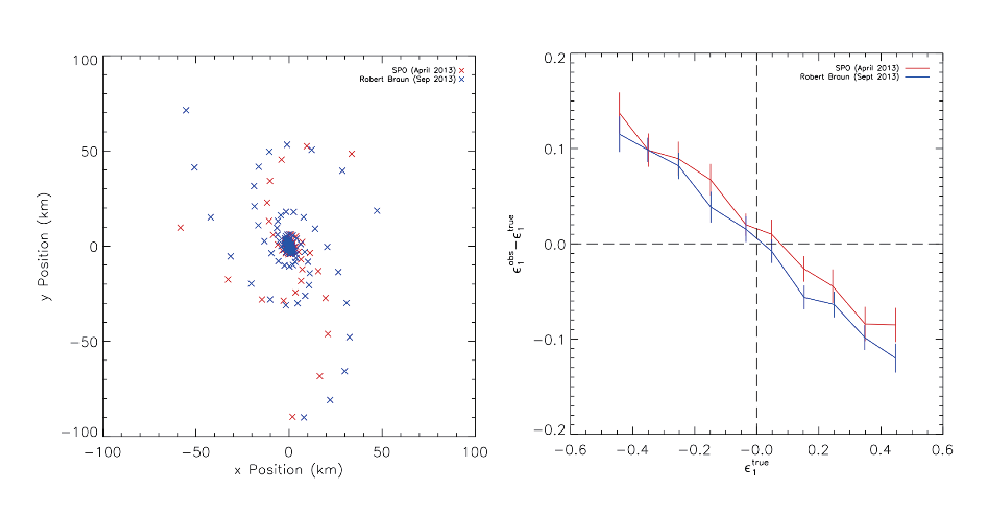
\includegraphics[width=0.95\linewidth]{cosmology/lensing_ellipse.eps} 
%   \vspace{10pt}
   \caption{SKAのアンテナ配置の違いによる、観測される銀河楕円率に生じる系統誤差の見積もり。
左図はアンテナの配置であり、右図は左図のそれぞれのアンテナ配置の場合に生じる
楕円率の系統誤差の大きさ(縦軸)を表す\cite{Patel:2015cra}。}\label{fig:weak_ellipse}
 \end{center}
\end{figure}
%%%%%%%%%%%%%%%%%%%%%%%%%%%%%%%%%%%%%%%%%%%%%%%%%%%%%%%%%%%%%%%%%%%%%%%%%%%%


また電波による弱重力レンズ効果の観測を行うことの利点として、
可視光観測との相関を取ることができるという点も挙げることが出来る。
例えば単一の観測(光学観測のみ等)によって測定された歪み場を$\gamma$とすると、
$\gamma$は重力レンズ起源の歪み場$\gamma_{\rm grav}$、その系統誤差$\gamma_{\rm sys}$
および銀河の固有の楕円率$\gamma_{\rm int}$によって
\begin{align}
	\gamma =\gamma_{\rm grav}+\gamma_{\rm int}+\gamma_{\rm sys}
	\,,
\end{align}
と表されるが、単にその自己相関を取った場合、
\begin{align}
	\langle\gamma\gamma\rangle
		=\langle\gamma_{\rm grav}\gamma_{\rm grav}\rangle
			+\langle\gamma_{\rm grav}\gamma_{\rm int}\rangle
			+\langle\gamma_{\rm int}\gamma_{\rm int}\rangle
			+\langle\gamma_{\rm sys}\gamma_{\rm sys}\rangle
	\,,
\end{align}
であり、系統誤差の寄与$\langle\gamma_{\rm sys}\gamma_{\rm sys}\rangle$が残ってしまうことになる。
次に電波観測と光学観測の間で相関を取ることを考えてみる。
電波観測による歪み場$\gamma^{(r)}$と光学観測による歪み場$\gamma^{(o)}$の間の相関を取ると
\begin{align}
	\langle\gamma^{(o)}\gamma^{(r)}\rangle
		=&\langle\gamma_{\rm grav}\gamma_{\rm grav}\rangle
			+\langle\gamma_{\rm grav}\gamma_{\rm int}^{(o)}\rangle
			+\langle\gamma_{\rm grav}\gamma_{\rm int}^{(r)}\rangle
			+\langle\gamma_{\rm int}^{(o)}\gamma_{\rm int}^{(r)}\rangle
			+\langle\gamma_{\rm sys}^{(o)}\gamma_{\rm sys}^{(r)}\rangle
	\notag\\
		=&\langle\gamma_{\rm grav}\gamma_{\rm grav}\rangle
			+\langle\gamma_{\rm grav}\gamma_{\rm int}^{(o)}\rangle
			+\langle\gamma_{\rm grav}\gamma_{\rm int}^{(r)}\rangle
			+\langle\gamma_{\rm int}^{(o)}\gamma_{\rm int}^{(r)}\rangle
	\,,
\end{align}
であり、第$5$項目の系統誤差の寄与を落とすことができる。
これは異なる実験間の系統誤差の間に相関がないということの結果である
($\langle\gamma_{\rm sys}^{(o)}\gamma_{\rm sys}^{(r)}\rangle =0$)。
また第$4$項である固有の楕円率の相関についても、電波と光学では放射機構が
異なるため、単一の観測のみの場合より小さくすることができる。
このように電波と可視光という異なる観測間で歪み場の相関を取ることによって、
両観測に存在する系統誤差等を取り除くことができるのである。
%その様な電波と可視光という異なる観測間で歪み場の相関を取ることによって、
%両観測に存在する系統誤差を取り除くことができるのである。
%
%

さらに電波観測においては、銀河の偏光の情報を利用できる
ということも大きな利点である。
%
銀河の弱重力レンズ効果を観測する上では、
銀河の元の楕円率の方向には相関が無いと仮定することで、
重力レンズによる楕円率の歪みの推定を行っている。
しかし実際には異なる銀河の楕円率の間には相関が存在しており、
その相関は系統誤差として影響を与える。
%
そこで、その元の銀河の楕円率の情報を得るために、
電波の偏光の情報を利用できるのではないかということが指摘されている。
この手法は銀河の元々の形状とその放射する電波の偏光との間に
相関が存在するため可能となる。
%
また銀河の回転軸と回転速度の観測を利用することで
元の銀河の方向を推定するという手法も提案されている。


%%%%%%%%%%%%%%%%%%%%%%%%%%%%%%%%%%%%%%%%%%%%%%%%%%%%%
\subsubsection{銀河楕円率推定のシミュレーション}
%
以上で説明した銀河の弱重力レンズ効果の観測においては、
ノイズの存在する観測データから、
銀河の形状(楕円率)を正確に推定することが重要となる。
%
そのため、銀河の楕円率を観測データから推定する解析手法の開発や、
電波干渉計のアンテナをどのように配置するのが、
銀河の楕円率を推定する上で最も効果的なのかについて、
詳細に調べていく必要が生じて来る。
%
そのことを目的とし、銀河の形状をインプットとして与え、
電波干渉計のアンテナ配置を様々に仮定した上で、
元の銀河の形をどの程度画像として正確に測定できるかについて
シミュレーションを行うという研究が現在行われている。
%
それらのシミュレーションでは、
アンテナ配置によって生じる系統誤差の大きさがどの程度になるのかについて
詳細に調べられており、そのシミュレーションによる結果の例が
図\ref{fig:weak_ellipse}の右図である。
% 
左図は計画されているSKAのアンテナの配置の一例で、
それぞれ赤と青の配置の場合に生じる系統誤差の影響が右図に示されている。
%
右図の縦軸はその系統誤差によって生じる
観測される銀河の楕円率の第1成分$\epsilon^{\rm obs}_{1}$と実際の銀河の楕円率$\epsilon^{\rm true}_{1}$の間の差を表している
(この図では楕円率の成分の内、片方の軸の成分のみ表示してある)。

今後、これら銀河の形状測定の妥当性がより詳細に検証されることが期待されており、
さらにこれらの手法を実際の電波干渉計のデータに用いることによる解析手法のテストについても、
将来のSKAによる弱重力レンズ効果の観測を目指して進展していくと予想される。



%%%%%%%%%%%%%%%%%%%%%%%%%%%%%%%%%%%%%%%%%%%%%%%%%%%%%%%%

\subsubsection{中性水素ガスの$21$cm線放射強度における重力レンズ効果}

これまでは銀河の形状に対する重力レンズ効果について述べてきたが、
さらにSKAではより大きな赤方偏移の時代
(宇宙再電離の時代から再電離が終わった後の時代にかけて)
を銀河間の中性水素ガスの$21$cm線輝線の観測によって
観測することが可能である。
したがって、その放射強度に対する弱重力レンズ効果についても
測定できると期待されている。
%
この観測における弱重力レンズ効果の測定手法は、
基本的にはCMBの重力レンズ効果観測における手法と同様であり、
歪み場の推定量を利用した統計的な解析を用いて、
弱重力レンズによる歪み場の測定を行うことが提案されてる。
%
この観測によって、銀河探査で観測できる時代より
さらに過去の密度揺らぎの情報を得ることが可能なため、
中性水素ガスの放射強度に対する弱重力レンズ効果の観測は、
暗黒エネルギーや修正重力理論の制限を目指す上で、
非常に有力な手法であると言うことができる。

%%%%%%%%%%%%%%%%%%%%%%%%%%%%%%%%%%%%%%%%%%%%%%%%%%%%

\bigskip

%%%%%%%%%%%%%%%%%%%%%%%%%%%%%%%%%%%%%%%%%%%%%%%%%%%%%
以上で説明してきた様に、
銀河の形状や中性水素の強度分布に対する弱重力レンズ効果の観測は、
SKAによる電波観測によって将来大きな進展が期待されており、
未だ詳細に調べられていない過去の宇宙を探査する上で、
非常に強力な観測手法となることが予想されている。



%%%%%%%%%%%%%%%%%%%%%%%%%%%%%%%%%%%%%%%%%%%%%%%%%%%%%%%%%%%%%%%%%%%%%%%%%%
\subsection{銀河団宇宙論}\label{cosmology.s2.ss7}
%%%%%%%%%%%%%%%%%%%%%%%%%%%%%%%%%%%%%%%%%%%%%%%%%%%%%%%%%%%%%%%%%%%%%%%%%%


%\subsubsection{Introduction}

中性水素$21$cm線は暗黒時代および再電離時期などを探るために
非常に有用な手段であることは様々に議論されているが~\citep{Pritchard:2011xb}、
ここでは、銀河団を用いた$21$cm線宇宙論について述べる。特に、銀河団による
スニヤエフ$\cdot$ゼルドヴィッチ(SZ)効果について考える~\citep{Colafrancesco2014}。

宇宙論的な$21$cm線放射が銀河団を通過する際、銀河団の中の
電子による逆コンプトン散乱で、そのスペクトルは変更を受ける。
これは、CMBでよく議論されているSZ効果であるが、
ここでは、特にこの宇宙論的な$21$cm線放射のスペクトルに関するこの効果を
SZ-$21$cm効果と呼ぶことにする。 

CMBの光子は銀河間物質を通過してくる際、
暗黒時代から、初代天体形成、再電離の時期において、
ガスとの衝突結合による吸収、
ライマン-$\alpha$、X線放射などにより、そのスペクトルは変更を受ける。
$I_0 (\nu)$ をCMBのスペクトルとし、
このスペクトルが銀河間物質を通過した後 $\widetilde{I}(\nu)$ に変更されたとすると、
宇宙論的な$21$cm線放射の(CMBに対する)輝度温度 $\delta T (\nu)$ は
\begin{equation}
%\label{ }
\delta T (\nu)
= \frac{c^2}{2 k_{\rm B} \nu^2} \left( \widetilde{I} (\nu) - I_0 (\nu) \right) 
= \frac{c^2}{2 k_{\rm B} \nu^2} \delta I (\nu)
\end{equation}
と書ける。ただし、ここでは レイリー$\cdot$ジーンズ周波数領域を考えている。

SZ-21cm効果は $\widetilde{I} (\nu)$ と $I_0 (\nu)$ それぞれに対するスニヤエフ$\cdot$ゼルドヴィッチ
効果の差として見ることができる。初期スペクトルが$\widetilde{I}(\nu) $ の放射について、
銀河団中の電子による逆コンプトン散乱の後、SZ効果によって変更されたスペクトルは
以下のように書ける~\citep{Cooray:2005bc}:
\begin{equation}
%\label{ }
\widetilde{I}_{\rm mod} (\nu) = \int_0^{\infty} d \nu_0 P_\tau (\nu, \nu_0) \widetilde{I} (\nu) 
\end{equation}
ここで、$P_\tau (\nu, \nu_0)$は振動数が$\nu_0$の光子が振動数$\nu$になる
確率を表す分布関数であり、散乱断面積、電子の分布関数、銀河団の光学的深さなどにより計算される。
特に一回の散乱による確率分布関数を$P_1(\nu, \nu_0)$とすると、光学的深さ$\tau$の銀河団を
通過した際は $P_\tau (\nu, \nu_0) = (1-\tau) \delta (\nu - \nu_0) + \tau P_1 (\nu, \nu_0)$と書ける
(ただし $\tau \ll 1$ とする)。
今考えているSZ-21cm効果は
\begin{equation}
\label{eq:SZE21cm}
\Delta I_{\rm mod} (\nu) = \widetilde{I}_{\rm mod} (\nu) - \widetilde{I} (\nu)
\end{equation}
に相当する。
電子が熱的、非熱的な分布をしている場合、それぞれを熱的SZ効果、非熱的SZ効果と呼ぶ。
%図\ref{fig:brightnessT}では熱的SZ効果の場合の振動数スペクトルが描かれている。

\subsubsection{SZ効果と$21$cm線}

ここでは実際の周波数スペクトルの理論予言について見てみる~\citep{Colafrancesco2014,Cooray:2005bc}。
図~\ref{fig:brightnessT}の左図はCMB放射に対する21cmの輝度温度で、
右図はその放射がさらに銀河団による熱的SZ効果を受けた後のスペクトルを示している。

まず、左図の輝度温度について、スペクトルの特徴的な振動数に着目して見てみる。
まず、$ 30 < z <200$ では衝突結合による吸収があり、
これに対応して$\nu \sim 20$~MHz を中心として、輝度温度が負になっている。
また、$ 20 <z <30$での初代天体からの ライマン-$\alpha$放射場による
吸収が $\nu\sim 70$~MHz で見られる。
そして、その後$z<20$での軟X線加熱により、$\nu\gtrsim 100\,$MHzで輝度温度が正に大きくなっている。

右図は左図のスペクトルと、そのスペクトルが銀河団による熱的SZ効果
を受けたあとのスペクトルとの差を取ったものである (\eqref{eq:SZE21cm}式に対応)。
このスペクトルも左図と同様に特徴的な振動数依存性があることがわかる。
特に、$\nu\sim 60$ MHzにライマン-$\alpha$放射場との相互作用による負のピークを持つが、
$z\sim 20$にライマン-$\alpha$の急激な吸収が起こることで$\nu\sim 70$ MHzに
正のピークを生成する。
右図のスペクトルを$21$cm線の観測で見る事ができれば、
銀河団サーベイに対して非常に有用である。
また、それらの銀河団の情報を通じて暗黒時代および再電離時期に関する情報が得られる。

また、図~\ref{fig:brightnessT}では熱的SZ効果によるものであるが、
同様にして非熱的な電子分布による非熱的SZ効果の場合の
振動数スペクトルも計算することができる~\citep{Colafrancesco2014}。
この非熱的SZ効果の方がその差$\Delta I_{\rm mod}$ は小さくなるが
(輝度温度$\delta T$ で$1/40$程度の大きさになる~\citep{Colafrancesco2014})、
そのスペクトルの形は熱的なものと異なるため、原理的にはそのスペクトルの違いに
より区別ができ、銀河団等の電子分布の情報を得る事ができる。

%%%%%%%%%Figure%%%%%%%%%%%%%%%%%%%%%%%%%%%%%%%%%%%%%%%%%%%%%%%%%%%%%%%%%%%%%
\begin{figure}[t]
 \begin{minipage}{0.5\hsize}
 \begin{center}
%   \vspace{15pt}
   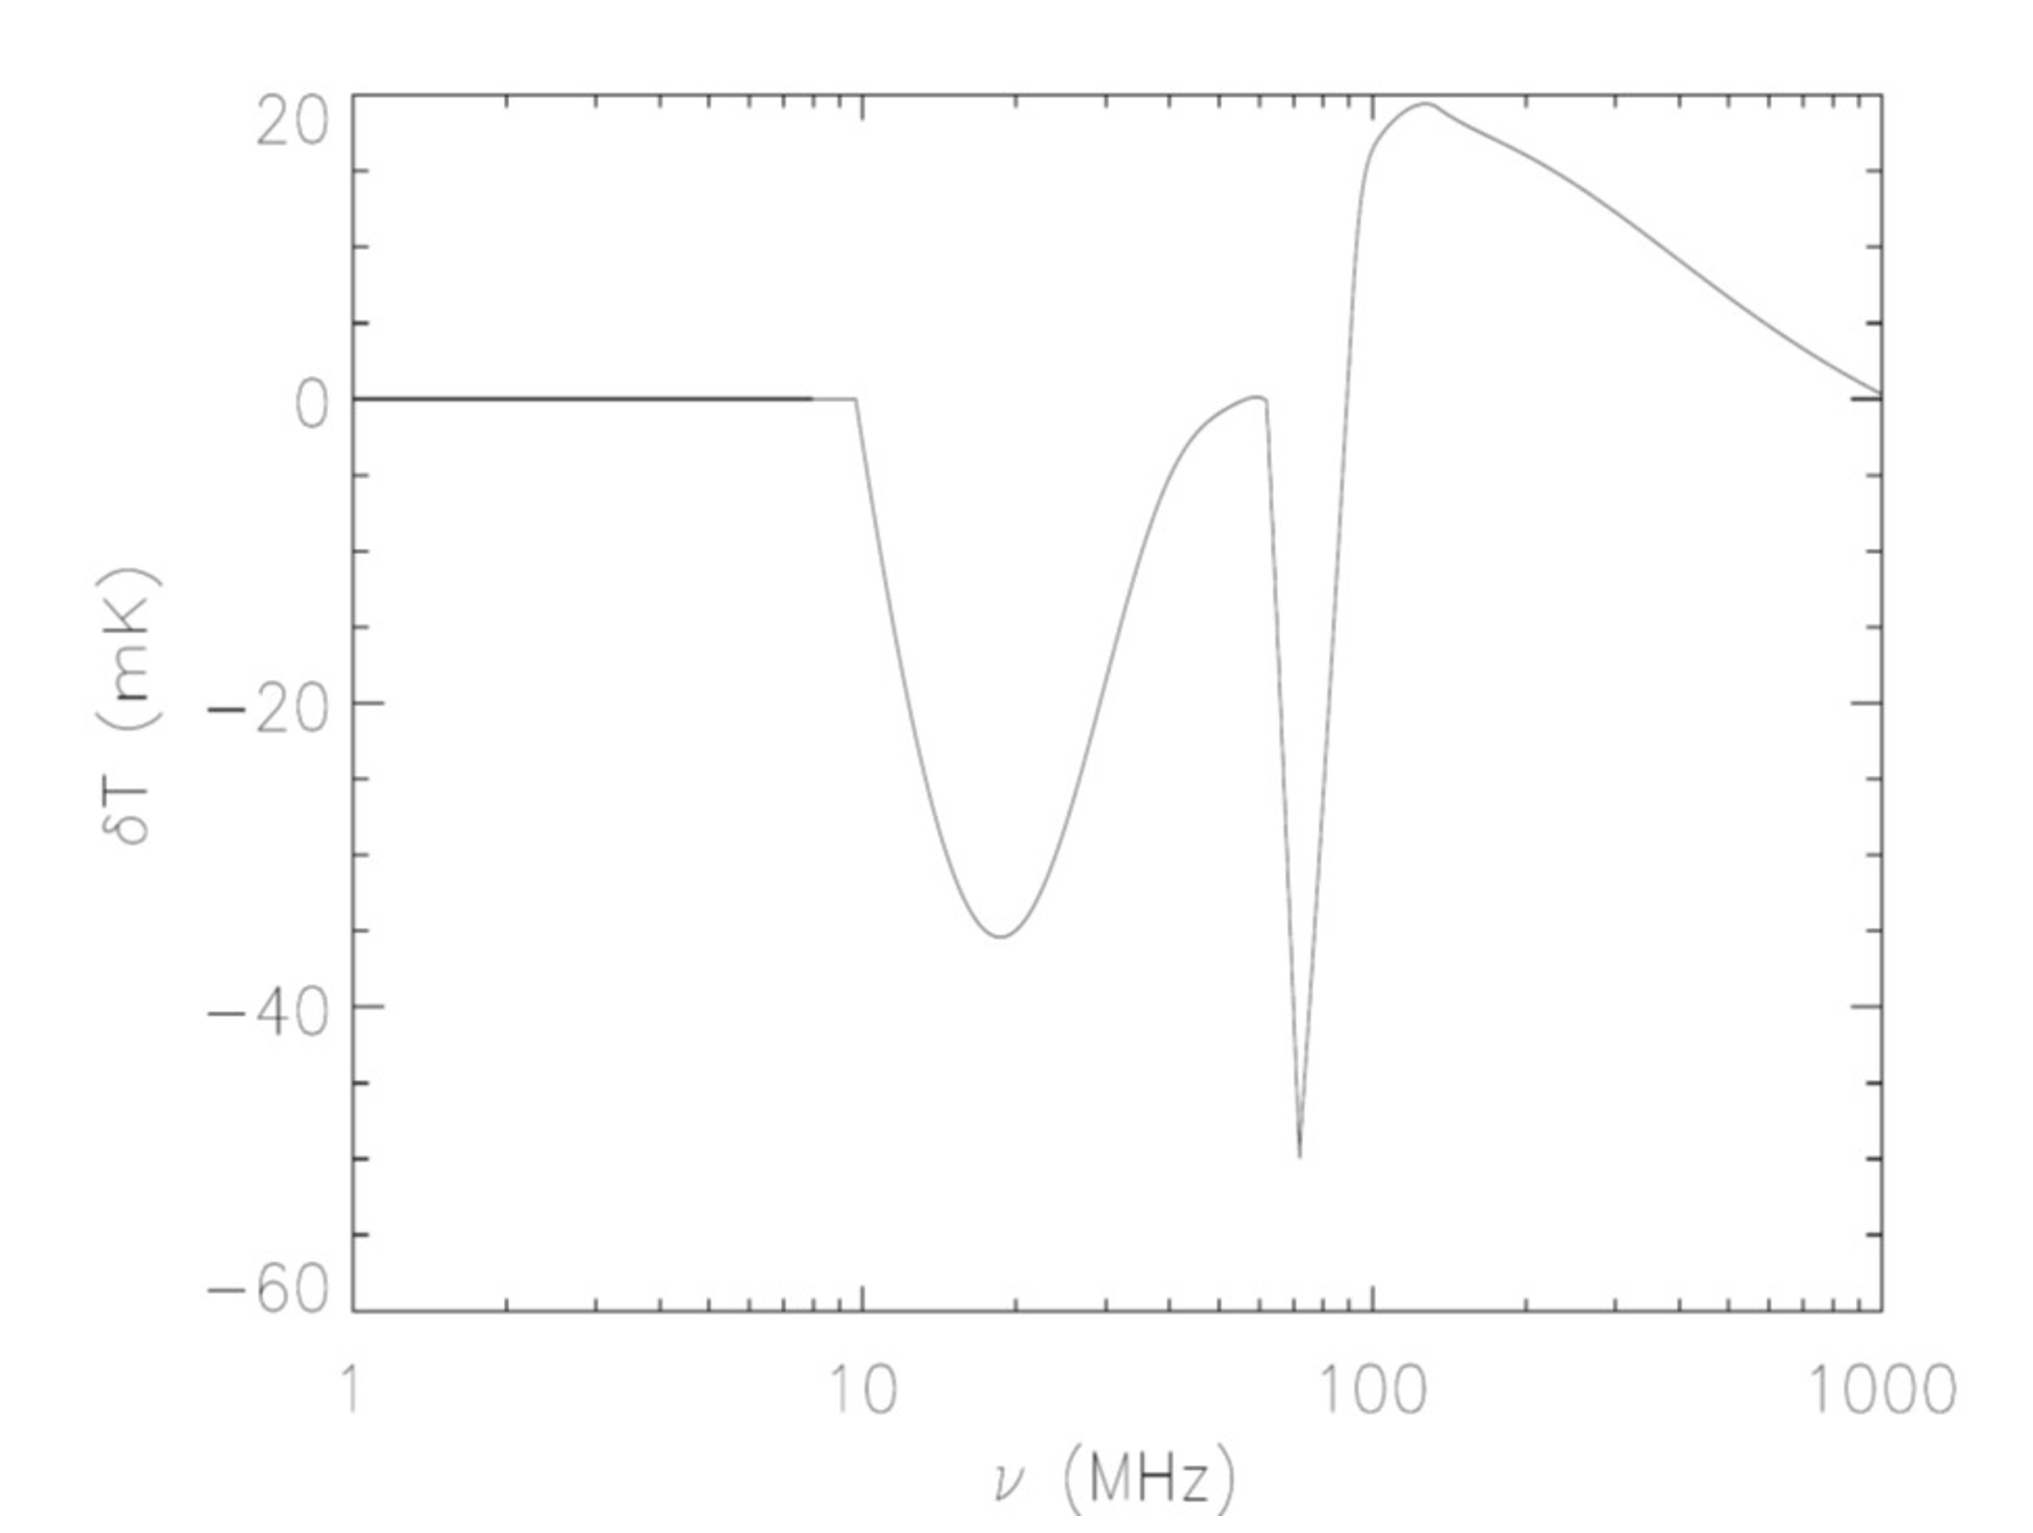
\includegraphics[width=1.0\linewidth]{cosmology/cluster_21cm.eps} 
%   \vspace{10pt}
 \end{center}
 \end{minipage}
 \begin{minipage}{0.5\hsize}
 \begin{center}
   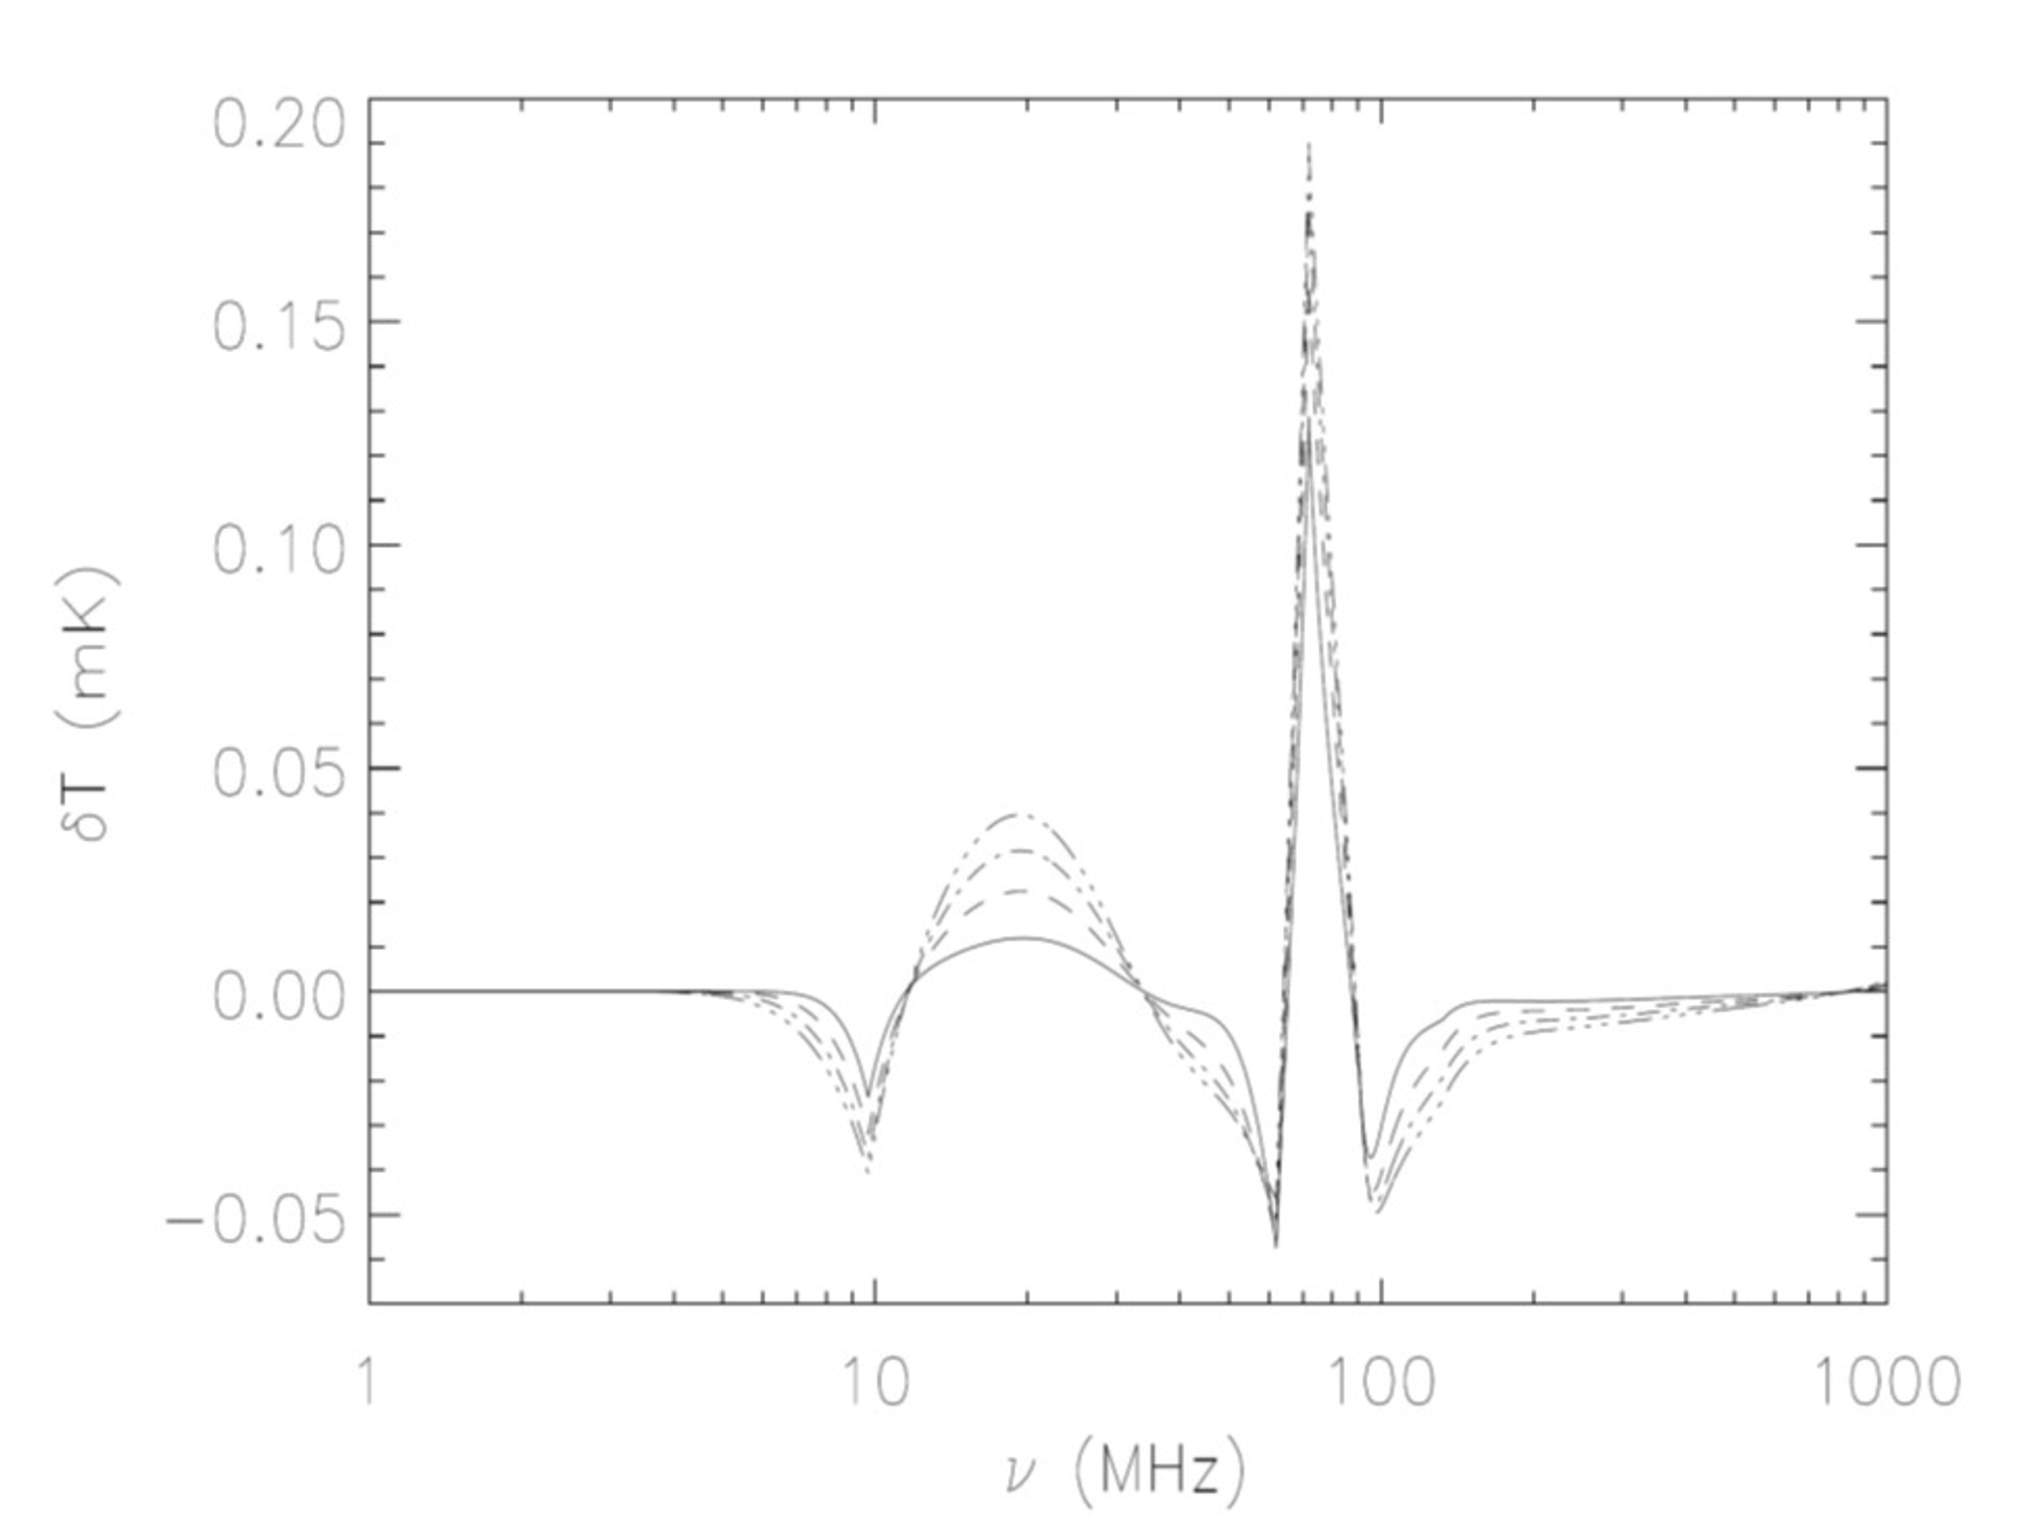
\includegraphics[width=1.0\linewidth]{cosmology/cluster_SZ-21cm.eps} 
%  \vspace{-15pt} 
 \end{center}
 \end{minipage}
\caption{(左図) CMB放射に対する輝度温度の周波数スペクトル。
(右図) 熱的SZ効果を受けた輝度温度スペクトルと受ける前のスペクトルの差。
熱的プラズマ温度はそれぞれ$kT = 5$ (solid) $10$ (dashed), $15$ (dotdashed), $20$ (dash-three dots) ${\rm keV}$
であり、光学的深さは$\tau =5\times 10^{-3}$としている\citep{Colafrancesco2014}。}
\label{fig:brightnessT} 
\end{figure}
%%%%%%%%%%%%%%%%%%%%%%%%%%%%%%%%%%%%%%%%%%%%%%%%%%%%%%%%%%%%%%%%%%%%%%%%%%%%


\subsubsection{SKAを用いた銀河団探査}

図~\ref{fig:brightnessT}より、熱的SZ-$21$cm効果のシグナルは振動数$300$~MHz以下で
大きくなることが分かる。
これは丁度SKA1-LOW ($50$--$250$~MHz) の振動数領域であり、
熱的SZ-$21$cm効果を観測するのに適していると言える。
実際、SZ-$21$cm効果を用いることで$\nu\sim 70$ MHzにおいては$kT\sim 20\,{\rm keV}$程度の
高温の銀河団、また、より高振動数側で感度が高くなるため、
$\nu\sim 90$ MHzにおいては比較的低温($kT\sim 5\,{\rm keV}$)程度の銀河団も
観測しうる。
一方、非熱的SZ-$21$cm効果のシグナルは(大きさは小さいものの)
SKA1-MID band 1 ($350$--$1050$~MHz) の方まで多少伸びているため、
このバンドでの観測可能性も興味深い。
これらのSZ-21cm効果のスペクトルを観測することにより、
対応する赤方偏移での暗黒時代、再電離時期を探査できる。

上記では、SZ-$21$cm効果を用いた暗黒時代、再電離時期の探査について述べたが、
銀河団を用いた宇宙論に関連するテーマとして、
ニュートリノ質量、暗黒エネルギー、修正重力理論、原始非ガウス性
なども議論できるであろう。



%%%%%%%%%%%%%%%%%%%%%%%%%%%%%%%%%%%%%%%%%%%%%%%%%%%%%%%%%%%%%%%%%%%%%%%%%%
\subsection{宇宙原理}\label{cosmology.s2.ss8}
%%%%%%%%%%%%%%%%%%%%%%%%%%%%%%%%%%%%%%%%%%%%%%%%%%%%%%%%%%%%%%%%%%%%%%%%%%

「我々の宇宙は空間的に一様かつ等方である」という宇宙原理の検証を高赤方偏移で
実現する可能性をSKAは秘めている。

現在の標準宇宙モデルに組み込まれつつあるインフレーション理論(\ref{cosmology.s1.ss1}節)において、
大きなスケールでの一様等方性は重要な予言である。インフレーション理論は、背景宇宙の
一様等方性を予言するだけでなく、CMBの温度揺らぎや、宇宙大規模構造の種となる初期密度揺らぎの起源を自然に説明できる。
そして、その予言される初期密度揺らぎの統計的性質は、ほぼガウス分布に従い、統計的に等方である、というものである。
さて、この宇宙原理の検証において、等方性の検証に比べ、一様性の検証はそれほど容易ではない~\citep{Ichiki:2014rua}。
CMB観測で温度がほぼ等方であることなどから、等方性は検証される。
さらに、CMB観測は、その温度揺らぎと偏光の情報からインフレーション理論を強く支持している。
しかし、
実は、すでにCMB観測で非常に大きなスケールでアノーマリーが見えているのでは、という議論があがっている。
温度揺らぎのパワーの大スケールでの欠損、そのパワーの双極子的な変調やパリティの非対称性などである。
これらアノーマリーが真に存在するのであれば、インフレーションを含めた標準宇宙モデルの変更を余儀なくされる。
よって、宇宙の一様等方性に関連した、これら非常に大きなスケールでのアノーマリーの精密な検証は、非常に重要である。
観測的には、CMBに比べ、SKAでは数多くの独立なモードを見ることが出来る。
大きなスケールに関して言えば、赤方偏移$z=O(1)$での超地平線のモードも見ることが可能である。
宇宙原理に関しては、例えばCMBと大規模構造の静止系が超地平線モードによって一致しない
可能性の検証が、SKAでは可能である~\citep{Schwarz:2015pqa}。

\subsubsection{宇宙論的な電波双極子} 

CMBにおけるダイポール(双極子)成分は、我々の固有運動のせいであると一般的には
「仮定」される。これにより、基準となるフレームを決めることになる。
しかし、厳密には運動起源の双極子なのか、他の物理現象からの双極子的寄与なのかを
CMBでは区別することが難しい。
すでに、電波観測で見られる双極子成分に対する制限は、NVSSやWENSSといった
電波源カタログから得られているが、いまだ誤差は大きい。CMB側では、
近年Planckチームにより、大きな多重極モーメントでも
ドップラーシフトの影響を発見したという報告もあったが、それほど精度が高いものでもない。
CMBの双極子成分の方向$\vec{d}_{\rm CMB}$と、電波源の双極子方向$\vec{d}_{\rm radio}$との
比較やその大きさ自体への制限にも、SKAの超地平線にわたる大きな体積での観測
が有効であると期待される。
具体的には、$< 1\,{\rm GHz}$の低周波数帯で連続波サーベイが有効であるが、
Early Science phaseで電波双極子の測定には十分である。

\subsubsection{大角度スケール}

運動学的起源の非等方性ではなく、時空そのものの等方性についての議論も、大きな角度スケールの観測により可能となる。
例えば、CMB観測では四重極と八重極揺らぎのパターン方向がそろっているなどのアノーマリーが報告されている。
SKAによる電波観測とCMB観測を組み合わせることで、観測されるCMB温度揺らぎを、最終散乱面で作られた成分と、
その後我々までに届く間に生まれた成分(例えば積分ザックス・ボルフェ効果)とに
分離できることが期待され、それによりアノーマリーの起源により詳細に迫ることが出来ると考えられる。

\begin{itemize}

\item 低い$\ell$多重極モーメント

これらアノーマリーに迫るためには、やはり大スケール、
つまり低$\ell$多重極モーメントの
精査が必要となる。図\ref{fig:low-ell}は、SKA1連続波サーベイで期待されるSKA銀河の角度パワースペクトルを誤差付きで表している。

\begin{figure}[tbp]\label{fig:fig.eps}
\begin{center}
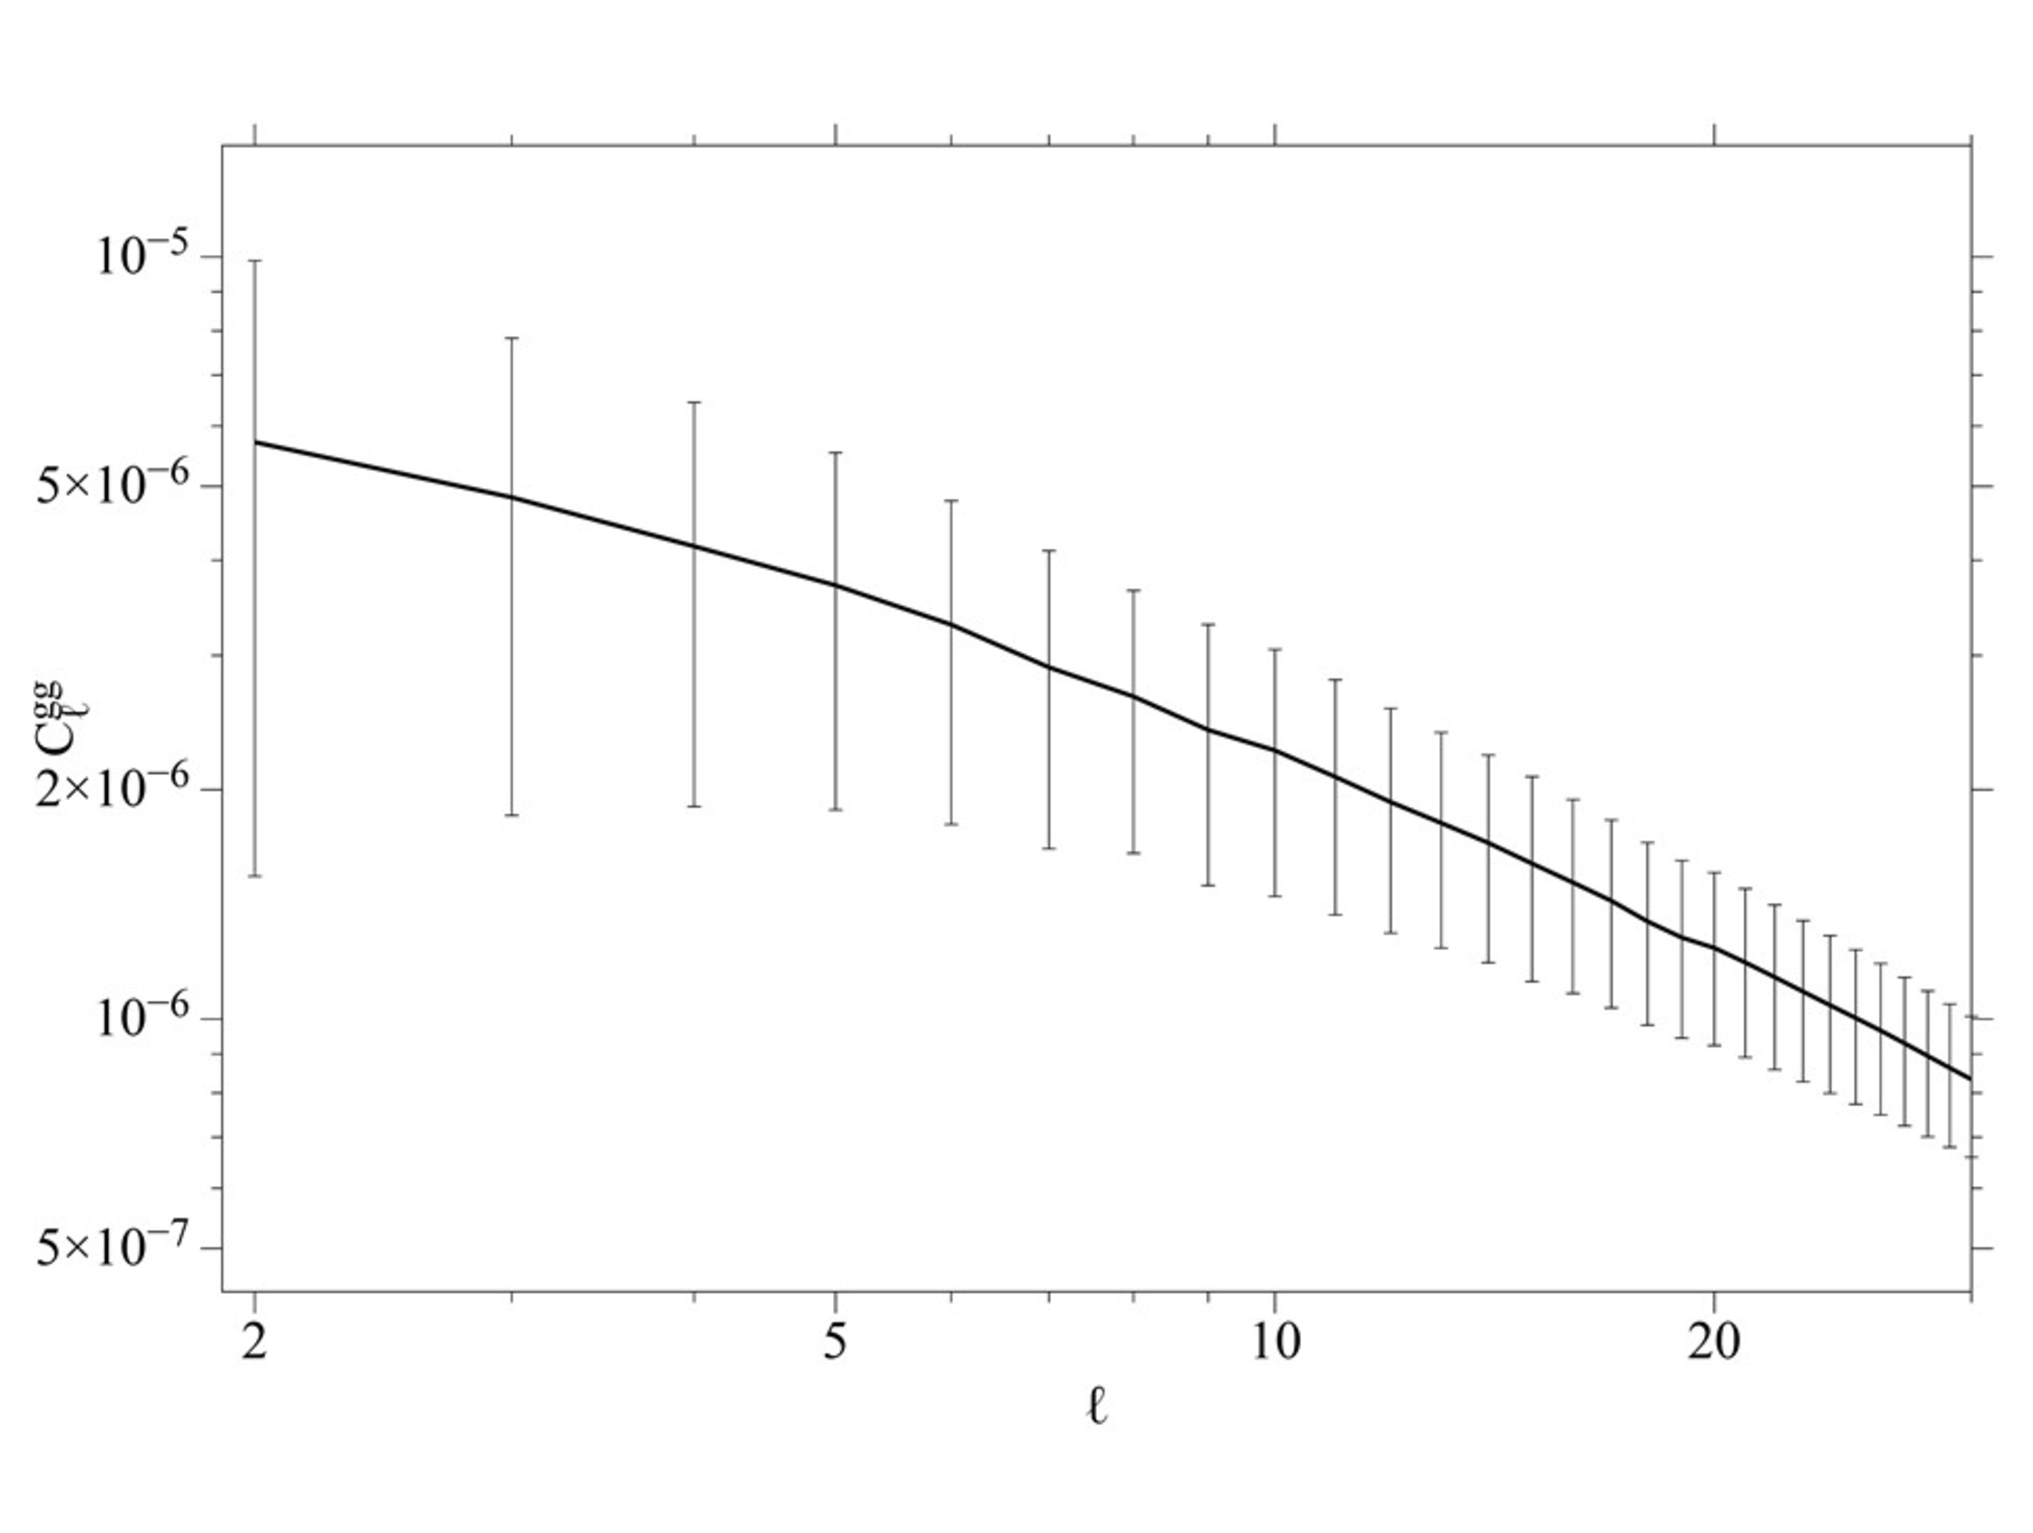
\includegraphics[width=0.6\linewidth]{cosmology/foundation_fig.eps}
\end{center}
\caption{SKA1連続波サーベイで期待されるSKA銀河の角度パワースペクトルとその観測誤差。}
  \label{fig:low-ell}
\end{figure}

\item 角度$2$点相関

大規模構造の分布を解析する際に、角度$2$点相関関数も有力な手法である。
原始揺らぎの非ガウス性への制限などにも角度$2$点相関関数は用いられている。
アノーマリーとは少し離れるが、大スケールの$2$点相関関数には、相対論的効果が
表れるという指摘もあり、とくに赤方偏移が分かるHI銀河赤方偏移サーベイにより、
この相対論的効果の検証も可能であると考えられる。

\end{itemize}

\subsubsection{コペルニクス原理と一様性}

コペルニクス原理とは、「我々がいる場所は宇宙の特別な空間ではない」というものである。
宇宙の等方性がわかって、この原理に従えば、宇宙の一様性が言えることになる。
コペルニクス原理の検証は、暗黒エネルギーの解明とも関連する。
宇宙が加速膨張していることを示唆する現在の観測結果を実現する
ためには、暗黒エネルギーの存在が不可欠であるがそれは一様性を仮定した時である。
コペルニクス原理が破れていて、我々が大きなボイド空間の中心にいても
宇宙が加速膨張しているように見える状況を作り出すことができるということも示唆されているが、
様々な観測との整合性を考えるとこのボイドモデルはあまりうまくいっていない。
しかし、その原理の検証をさらに詳細に行うことは重要である。
一様か一様でないかのチェックとして、
\begin{equation}
{\mathcal C}(z) = 1 + \widetilde h^2\left( DD'' - {D'}^2\right) + \widetilde h\widetilde h' DD' = 0
\end{equation}
という式を用いることができる~\citep{Clarkson:2007pz}。ここで、$\widetilde h= H(z) / H_0 $、$D(z)$
は共動距離を表し、また$' = d/dz$である。
${\mathcal C}(z) \neq 0$でコペルニクス原理が破れていることを表す。
SKA1では、$z<1.5$の観測データを用いて$\sigma ({\mathcal C}(z)) =0.05$まで到達可能であると期待される。
\\

現代の宇宙論は、飛躍的な観測技術の進歩により、精密科学の域にまで達している。
今後は、これまで仮定としていた宇宙の一様性、等方性という宇宙論の基礎の検証も出来ると考えられている。
CMB観測と合わせて、SKAによる電波観測もその有力な道具の一つとして期待される。



